%% For double-blind review submission, w/o CCS and ACM Reference (max submission space)
%\documentclass[sigplan,review,anonymous]{acmart}\settopmatter{printfolios=true,printccs=false,printacmref=false}
\documentclass[sigplan,10pt,review,anonymous]{acmart}\settopmatter{printfolios=true,printccs=false,printacmref=false}
%% For double-blind review submission, w/ CCS and ACM Reference
%\documentclass[sigplan,review,anonymous]{acmart}\settopmatter{printfolios=true}
%% For single-blind review submission, w/o CCS and ACM Reference (max submission space)
%\documentclass[sigplan,review]{acmart}\settopmatter{printfolios=true,printccs=false,printacmref=false}
%% For single-blind review submission, w/ CCS and ACM Reference
%\documentclass[sigplan,review]{acmart}\settopmatter{printfolios=true}
%% For final camera-ready submission, w/ required CCS and ACM Reference
%\documentclass[sigplan]{acmart}\settopmatter{}


%% Conference information
%% Supplied to authors by publisher for camera-ready submission;
%% use defaults for review submission.
\acmConference[PL'18]{ACM SIGPLAN Conference on Programming Languages}{January 01--03, 2018}{New York, NY, USA}
\acmYear{2018}
\acmISBN{} % \acmISBN{978-x-xxxx-xxxx-x/YY/MM}
\acmDOI{} % \acmDOI{10.1145/nnnnnnn.nnnnnnn}
\startPage{1}

%% Copyright information
%% Supplied to authors (based on authors' rights management selection;
%% see authors.acm.org) by publisher for camera-ready submission;
%% use 'none' for review submission.
\setcopyright{none}
%\setcopyright{acmcopyright}
%\setcopyright{acmlicensed}
%\setcopyright{rightsretained}
%\copyrightyear{2018}           %% If different from \acmYear

%% Bibliography style
\bibliographystyle{ACM-Reference-Format}
%% Citation style
%\citestyle{acmauthoryear}  %% For author/year citations
%\citestyle{acmnumeric}     %% For numeric citations
%\setcitestyle{nosort}      %% With 'acmnumeric', to disable automatic
                            %% sorting of references within a single citation;
                            %% e.g., \cite{Smith99,Carpenter05,Baker12}
                            %% rendered as [14,5,2] rather than [2,5,14].
%\setcitesyle{nocompress}   %% With 'acmnumeric', to disable automatic
                            %% compression of sequential references within a
                            %% single citation;
                            %% e.g., \cite{Baker12,Baker14,Baker16}
                            %% rendered as [2,3,4] rather than [2-4].


%%%%%%%%%%%%%%%%%%%%%%%%%%%%%%%%%%%%%%%%%%%%%%%%%%%%%%%%%%%%%%%%%%%%%%
%% Note: Authors migrating a paper from traditional SIGPLAN
%% proceedings format to PACMPL format must update the
%% '\documentclass' and topmatter commands above; see
%% 'acmart-pacmpl-template.tex'.
%%%%%%%%%%%%%%%%%%%%%%%%%%%%%%%%%%%%%%%%%%%%%%%%%%%%%%%%%%%%%%%%%%%%%%


%% Some recommended packages.
\usepackage{booktabs}   %% For formal tables:
                        %% http://ctan.org/pkg/booktabs
\usepackage{subcaption} %% For complex figures with subfigures/subcaptions
                        %% http://ctan.org/pkg/subcaption
%% Custom Packages
\usepackage[T1]{fontenc}
\usepackage{listings}
\usepackage{color}
\usepackage{xspace}
\usepackage[title]{appendix}
%\usepackage{tikz}
%\usepackage{pgf-pie}
\usepackage{forest}
\usepackage{amsmath,amssymb}
\usepackage{ctable}
\usepackage[textsize=tiny]{todonotes}
\usepackage{pifont}
\usepackage{calculator}
\usepackage{csquotes}
%\usepackage[ruled,vlined]{algorithm2e}
%\usepackage{algorithm}
%\usepackage{algorithmic}
\usepackage[linesnumbered,ruled]{algorithm2e}

% opphans
\clubpenalty = 10000
\widowpenalty = 10000
\displaywidowpenalty = 10000

%\setlength{\parskip}{0.5pt plus 4pt minus 3pt}
%\setlength{\textfloatsep}{1\baselineskip plus 0.2\baselineskip minus 0.5\baselineskip}
\newenvironment{tightcenter}{%
    \setlength\topsep{4pt}
    \setlength\parskip{-2pt}
    \begin{center}
    }{%
    \end{center}
}

% FIXME: overleaf broken if uncommented
\usepackage{tikz}
\usetikzlibrary{shapes,arrows,shadows,backgrounds}
\usetikzlibrary{arrows.meta}
\usepackage{amsmath,bm,times}

%% Custom Commands
\def\Code#1{\texttt{#1} }
%\def\Comment#1{}
\def\Comment#1{\textbf{\textsl{\color{red}  $\langle\!\langle$#1$\rangle\!\rangle$}} }
\newcommand{\percentage}[2]{\DIVIDE{#1}{#2}{\duv}\MULTIPLY{\div}{100}{\res}$\res\%$}
\newcommand{\revisit}[1]{{\color{red} Sandeep: #1}}
\newcommand{\Qd}[1]{{\color{red} Daejun: #1}}
\newcommand{\Qt}[1]{{\color{red} Theo: #1}}
\newcommand{\BW}[1]{{\color{red} Borrowed: #1}}
\newcommand{\Added}[1]{{\color{red} #1}}
%\newcommand{\SC}[1]{{\color{blue} #1}}
%\newcommand{\AEC}[1]{{\color{blue} #1}}
\newcommand{\SC}[1]{#1}
\newcommand{\AEC}[1]{#1}
\newcommand{\cmt}[1]{}
\newcommand{\xmark}{{\color{red} \ding{55}}}
\newcommand{\cmark}{{\color{green} \ding{51}}}
\newcommand{\ISA}{x86-64\xspace}
\newcommand{\LLVM}{LLVM IR\xspace}
\newcommand{\compd}{Compositional Lifter\xspace}
\newcommand{\siv}{single-instruction validation\xspace}
\newcommand{\Siv}{Single-instruction validation\xspace}
\newcommand{\plv}{program-level validation\xspace}
\newcommand{\tv}{translation validation\xspace}
\newcommand{\Mcstate}{\emph{State}\xspace}
%\newcommand{\K}{\mbox{$\mathbb{K}$}\xspace}
\newcommand{\Z}{$\mathbb{Z}3$\xspace}
\newcommand{\mcsema}{McSema\xspace}
\newcommand{\dlifted}{McSema-lifted\xspace}
\newcommand{\uif}{uninterpreted functions}
\newcommand{\TV}{Translation Validation\xspace}
\newcommand{\syncps}{synchronization points\xspace}
\newcommand{\syncp}{synchronization point\xspace}
\newcommand{\Strata}{Strata\xspace}
\newcommand{\Stoke}{Stoke\xspace}
\newcommand{\initS}{{\tt initial search}}
\newcommand{\secS}{{\tt secondary searches}}
%\newcommand{\K}{\ensuremath{\mathcal{{\tt K}}}\xspace}
\newcommand{\TS}[1]{{\tt #1}}
\newcommand{\matcher}{Matcher\xspace}
%\newcommand{\instr}[1]{\texttt{#1}}
\newcommand{\instr}[1]{\textbf{\color{brown}\m{#1}}}
\newcommand{\reg}[1]{\texttt{\%#1}}
\newcommand{\mem}[2]{\texttt{#1(\%#2)}}
\newcommand{\opcode}[1]{\ensuremath{#1}}
%\newcommand{\cond}[1]{\ensuremath{#1}}
\newcommand{\extract}{\emph{extract}\xspace}
\newcommand{\extractMInt}{\emph{extractMInt}\xspace}
\newcommand{\false}{\textbf{False}}
\newcommand{\true}{\textbf{True}}
\newcommand{\bool}{\texttt{Bool}\xspace}
\newcommand{\incfig}[1]{\includegraphics[scale=.7]{#1}}
\newcommand{\CF}[2]{$\s{F}_{\s{#2}}^{\s{#1}}$}
%\newcommand{\GN}[2]{$G{[#2]}^{#1}$}
\newcommand{\udef}{\emph{undef}\xspace}
\newcommand{\bv}[2]{$#1\text{'}#2$\xspace}
%% Graph algo
\newcommand{\N}{\s{N}\xspace}
\newcommand{\NP}{\s{N$^\prime$}\xspace}

\newcommand{\T}{\s{T}\xspace}
\newcommand{\TP}{\s{T$^\prime$}\xspace}

\newcommand{\un}{$u$\xspace}
\newcommand{\vn}{$v$\xspace}
\newcommand{\up}{$u^\prime$\xspace}
\newcommand{\IN}{\s{I$_{N}$}\xspace}
\newcommand{\INP}{\s{I$_{N^\prime}$}\xspace}
\newcommand{\F}{\s{F}\xspace}
\newcommand{\FP}{\s{F$^\prime$}\xspace}
\newcommand{\FN}{\s{F$_{N}$}\xspace}
\newcommand{\FNP}{\s{F$_{N}^\prime$}\xspace}
\newcommand{\GN}{\s{G$_{\FN}$}\xspace}
\newcommand{\GNP}{\s{G$_{\FNP}$}\xspace}
\newcommand{\Ap}{\s{A$^\prime$}\xspace}
\newcommand{\Bp}{\s{B$^\prime$}\xspace}
\newcommand{\Dp}{\s{D$^\prime$}\xspace}
\newcommand{\Lp}{\s{L$^\prime$}\xspace}
\newcommand{\Np}{\s{N$^\prime$}\xspace}
\newcommand{\Sp}{\s{S$^\prime$}\xspace}
\newcommand{\Tp}{\s{T$^\prime$}\xspace}

\newcommand{\pot}{$\phi$\xspace}
\newcommand{\potp}{\s{$\phi^\prime$}\xspace}
\newcommand{\potpup}{$\phi^\prime$(\up)\xspace}
\newcommand{\potvup}{$\phi_{v}$(\up)\xspace}
\newcommand{\potu}{$\phi$(\un)\xspace}
\newcommand{\potup}{$\phi$(\up)\xspace}

%%

\newcommand{\rating}[1]{%
    \begin{tikzpicture}[x=1ex,y=1ex]
    \begin{scope}
    \clip (0,1) circle (1);
    \fill[black] (-1,0) rectangle (1,#1/50);
    \end{scope}
    \draw[black, thin, radius=1] (0,1) circle;
    \end{tikzpicture}%
}

% Current Support
\newcommand{\currentIS}{$3155$\xspace}
\newcommand{\currentIntel}{$774$\xspace}
% Total
\newcommand{\totalIS}{$3736$\xspace}
\newcommand{\totalIntel}{$996$\xspace}
\newcommand{\dup}{$109$\xspace}
% Mcsema
\newcommand{\mcsemaIS}{$1922$\xspace}
%
\newcommand{\plvT}{$2348$\xspace}
\newcommand{\plvP}{$2189$\xspace}
%
\newcommand{\sivIS}{$1349$\xspace}
\newcommand{\sivExc}{$573$\xspace}
\newcommand{\sivFail}{$29$\xspace}
\newcommand{\sivTO}{$6$\xspace}
%
% Strata
\newcommand{\strataIS}{$1796$}
\newcommand{\strataIntel}{$466$}
\newcommand{\strataWithDupIS}{$1905$}
\newcommand{\strataRegVarIS}{$692$}
% Unsupported
\newcommand{\system}{$210$}
\newcommand{\Xmmx}{$336$}
\newcommand{\crypto}{$35$}

\newcommand{\strataPerc}{$47\%$} % 466/996 or  1905 / 3736
\newcommand{\goelPerc}{$33\%$} 
\newcommand{\sailPerc}{$15\%$} 
% Stoke disjoin from Strata
%\newcommand{\stokeIS}{$332$} % 262 + 15 + 9 + 46. ALso 332/3767 == 9%
% 1432(strata common) + 332
\newcommand{\stokeIS}{${\sim}1764$}
%\newcommand{\stokeExcPerc}{$9\%$}
% Strata stoke combined
%\newcommand{\strataPlusStokeIS}{$2237$} % 

%\newcommand{\unsupp}{$939$}

%%%%%% Immediates
%\newcommand{\ImmUg}{$146$} % 118 + 28
%\newcommand{\ImmTotal}{$308$}
%\newcommand{\ImmG}{$190$}

%%%%%%% Registers
%\newcommand{\RegTOTAL}{$1133$} % 1083 + 50
%\newcommand{\RegSTRAT}{$742$} % 692 + 50
%\newcommand{\RegSTOK}{$262$}
%\newcommand{\RegMAN}{$129$}

%%% toture status
\newcommand{\TortureTotal}{$1576$} %
\newcommand{\TortureExclude}{$6$} % 6 + 22
\newcommand{\TortureInclude}{$1548$}
\newcommand{\TortureUifsInstr}{$293$} % 134(all three jobs) +  48
\newcommand{\TortureUifs}{$35$}
\newcommand{\TortureCoverage}{$963$}
%%% Undef counts
\newcommand{\undefTotal}{$474$}
\newcommand{\undefIntel}{$32$}
\newcommand{\undefPerc}{$3$} %32/1000

\PassOptionsToPackage{pdftex,usenames,dvipsnames,svgnames,x11names}{xcolor}
\PassOptionsToPackage{pdftex}{hyperref}
\usepackage[style=math]{k}


% Slightli modified original version of \reduce. Altered baseline for more compactness.
% No support for multiline.
\newcommand{\reduceClassic}[2]{\hbox{%
  \begin{tikzpicture}[baseline=(top.south), %(top.base), - default, less compact
                      inner xsep=0pt,
                      inner ysep=.3333ex,
                      minimum width=2em]
    \path
          % Original version. No support for line wrapping.
          node (top) [inner ysep=1ex]{$#1$ \mathstrut}

          % New version. Line wrapping support.
          %node (top) [inner ysep=1ex]{$ \begin{array}{@{}c@{}} #1 \end{array} $ \mathstrut}
          (top.south)
          % Original version. No support for line wrapping.
          node (bottom) [anchor=north, inner ysep=.5ex] {$#2$};

          % New version. Line wrapping support.
          % Adds a little bit of vertical space, but the difference is truly insignificant. All the experiments below failed to remove it.
          %node (bottom) [anchor=north, inner ysep=.5ex] {$ \begin{array}{@{}c@{}} #2 \end{array} $};
          % no extra effect
          % node (bottom) [anchor=north, inner ysep=.5ex] {\vspace{-1em} $ \begin{array}{@{}c@{}} #2 \end{array} $};
          % trying mathstrut - some horizontal re-alignment, but no vertical
          % node (bottom) [anchor=north, inner ysep=.5ex] {$ \begin{array}{@{}c@{}} #2 \end{array} $ \mathstrut};
          % no outer ysep (if no inner - looks bad)
          %node (bottom) [anchor=north, inner ysep=.5ex, outer ysep=0] {$ \begin{array}{@{}c@{}} #2 \end{array} $};
          % \vskip -1em just don't compile no matter where we put it
    \path[draw,thin,solid] let \p1 = (current bounding box.west),
                               \p2 = (current bounding box.east),
                               \p3 = (top.south)
                           in (\x1,\y3) -- (\x2,\y3);
    % Solid arrow (augmenting the solid line).
    \path[fill] (top.south) ++(2pt,0) -- ++(-4pt,0) -- ++(2pt,-1.5pt) -- cycle;
  \end{tikzpicture}%
}}

% Defalut version of \reduce in this document.
%   Support for multi-line LHS and RHS
%   Good compactness. Separators adjusted to be aligned with \reduceClassic
\newcommand{\reduceMulti}[2]{\hbox{%
  \begin{tikzpicture}[baseline=(top.south), %(top.base), - default, less compact
                      inner xsep=0pt,
                      inner ysep=.3333ex,
                      minimum width=2em]
    \path
          % New version. Line wrapping support.
          node (top) [
            %inner ysep=1ex
            inner ysep=0.6ex
          ]{ $ \begin{array}{@{}c@{}}
                #1
               \end{array} $ \mathstrut}
          (top.south)
          % New version. Line wrapping support.
          node (bottom) [
            anchor=north,
            %inner ysep=.5ex
          ] {
            $ \begin{array}{@{}c@{}}
              #2
            \end{array} $};
    \path[draw,thin,solid] let \p1 = (current bounding box.west),
                               \p2 = (current bounding box.east),
                               \p3 = (top.south)
                           in (\x1,\y3) -- (\x2,\y3);
    % Solid arrow (augmenting the solid line).
    \path[fill] (top.south) ++(2pt,0) -- ++(-4pt,0) -- ++(2pt,-1.5pt) -- cycle;
  \end{tikzpicture}%
}}

%Special version of \reduce with modified baseline, for better rendering of multiline
% LHS and RHS
\newcommand{\reduceCompact}[2]{\hbox{%
  \begin{tikzpicture}[baseline=(bottom), %(top.base), - default, less compact
                      inner xsep=0pt,
                      inner ysep=.3333ex,
                      minimum width=2em]
    \path
          node (top) [inner ysep=0.6ex]{$ \begin{array}{@{}c@{}} #1 \end{array} $ \mathstrut}
          (top.south)
          node (bottom) [anchor=north] {$ \begin{array}{@{}c@{}} #2 \end{array} $};
    \path[draw,thin,solid] let \p1 = (current bounding box.west),
                               \p2 = (current bounding box.east),
                               \p3 = (top.south)
                           in (\x1,\y3) -- (\x2,\y3);
    % Solid arrow (augmenting the solid line).
    \path[fill] (top.south) ++(2pt,0) -- ++(-4pt,0) -- ++(2pt,-1.5pt) -- cycle;
  \end{tikzpicture}%
}}

%\renewcommand{\reduce}[2]{\reduceClassic{#1}{#2}}
\renewcommand{\reduce}[2]{\reduceMulti{#1}{#2}}




%\lstset{captionpos=t,tabsize=3,frame=no,keywordstyle=\color{blue},
%        commentstyle=\color{gray},stringstyle=\color{red},
%        breaklines=true,showstringspaces=false,emph={label},
%        basicstyle=\ttfamily}

% Required in order to make \kall cells inside comments black.
\renewcommand{\kall}[3][black]{\mall{#1}{#2}{#3}}

% Environment "kdefinition" has effect only in poster style, thus in math style may be safely deleted.

%Continuation of a syntax definition on a new line
\newcommand{\syntaxContNewLine}[3][\defSort]{\par\indent\rulebox{%
  $\setlength{\syntaxlength}{\widthof{$\mathrel{::=}$}}%
  \setlength{\syntaxlength}{.5\syntaxlength}%
  \addtolength{\syntaxlength}{\widthof{\syntaxKeyword$#1$}}%
  \hspace{\syntaxlength}%
  \;\;\;\;\;\;\;{#2}$ \ifthenelse{\equal{#3}{}}{}{[#3]}%
  }%\k@markPosition%
}

%Should be put after a syntaxLong.
\newcommand{\syntaxEnd}[3][\defSort]{
  \indent\rulebox{%
  $\setlength{\syntaxlength}{\widthof{$\mathrel{::=}$}}%
  \setlength{\syntaxlength}{.5\syntaxlength}%
  \addtolength{\syntaxlength}{\widthof{\syntaxKeyword$#1$}}%
  \hspace{\syntaxlength}$%
  }%\k@markPosition%
}

\newcommand{\syntaxLong}[3][\defSort]{\rulebox{%
\syntaxKeyword
$
  \begin{array}[t]{@{}l@{}}
  #1 \\
  \mathrel{::=}{#2}
  \end{array}
$ {}%
}%\k@markPosition%
}

% Grigore's idea macro
\newcommand{\idea}[1]{
  \begin{quote}
    \rule{.45\textwidth}{.5pt}\newline
    {\em #1}
    \vspace*{-1ex}\newline \rule{.45\textwidth}{.5pt}
  \end{quote}
}

\newenvironment{ideas}
{ \begin{quote}
    \rule{.45\textwidth}{.5pt}
    \newline
    \begin{em}
} {
    \end{em}
    \vspace*{-1ex}
    \leavevmode
    \newline
    \rule{.45\textwidth}{.5pt}
  \end{quote}
}

%Enforcing black cells
\renewcommand{\kall}[3][white]{\mall{black}{#2}{#3}}
\renewcommand{\kallLarge}[3][white]{\mallLarge{black}{#2}{#3}}
\renewcommand{\kprefix}[3][white]{\mprefix{black}{#2}{#3}}
\renewcommand{\ksuffix}[3][white]{\msuffix{black}{#2}{#3}}
\renewcommand{\kmiddle}[3][white]{\mmiddle{black}{#2}{#3}}

% Settigns required for Chucky's background section
\usepackage{acronym}

\providecommand{\Sec}{}
\renewcommand{\Sec}{Section~}
\newcommand{\Fig}{Figure~}

\newcommand{\cellname}[1]{\textsf{#1}}

\newcommand{\kequation}[2]{\begin{equation*}{\small#2}\end{equation*}}

%Probably a mapsto with spacing
\newcommand{\mapstox}{\small\mathrel{\mapsto}}

%For spacing between cell lines
%\newcommand{\kBR}{\\[0.3em]}

% General
\newcommand{\w}[1]{\ensuremath{\textit{#1}}}
\newcommand{\m}[1]{\ensuremath{\texttt{#1}}}
\newcommand{\s}[1]{\ensuremath{\textsf{#1}}}
\newcommand{\p}[1]{\ensuremath{\left(#1\right)}}
\newcommand{\pl}[1]{\ensuremath{\left\langle#1\right\rangle}}
\newcommand{\OR}{\mbox{ }|\mbox{ }}
\newcommand{\st}{.\mbox{ }}
\newcommand{\finto}{\ensuremath{\stackrel{\mathtt{fin}}{\longrightarrow}}}
\newcommand{\defeq}{\ensuremath{\stackrel{\mathtt{def}}{=}}}
\newcommand{\cond}[1]{\ensuremath{\left\{\begin{array}{ll} #1 \end{array}\right.}}
\newcommand{\lst}[1]{\begin{itemize} {#1} \end{itemize}}
\newcommand{\pby}[1]{\hspace*{\fill}{#1}}
\newcommand{\slide}[2][]{ \begin{frame} \frametitle{#1} {#2} \end{frame} }
\newcommand{\etal}{\textit{et~al.}\xspace}

% For references
\newcommand{\fig}[1]{Figure~\ref{#1}}
\newcommand{\lem}[1]{Lemma~\ref{#1}}
\newcommand{\theo}[1]{Theorem~\ref{#1}}
\newcommand{\coro}[1]{Corollary~\ref{#1}}
\newcommand{\defn}[1]{Definition~\ref{#1}}
\newcommand{\rmrk}[1]{Remark~\ref{#1}}
\newcommand{\exam}[1]{Example~\ref{#1}}
\newcommand{\sect}[1]{$\S$~\ref{#1}}

%\newcommand{\todo}[1]{}
%\newcommand{\todo}[1]{{\textcolor{red}{\textbf{[[{#1}]]}}}}

\usepackage{ucs} % for unicode characters (just for \Rosu and \Serbanuta)
\newcommand{\sh}{\unichar{0537}}
\newcommand{\Sh}{\unichar{0536}}
\PrerenderUnicode{\sh}
\PrerenderUnicode{\Sh}
\newcommand{\Rosu}{Ro{\sh}u\xspace}
\newcommand{\Stefanescu}{{\Sh}tef{\u a}nescu\xspace}

\newcommand{\JS}{JavaScript\xspace}
\newcommand{\ES}{ECMAScript\xspace}
%\newcommand{\K}{\ensuremath{\mathbb{K}}\xspace}
%\newcommand{\KJS}{\ensuremath{\mathbb{K}}JS\xspace}
\newcommand{\KJS}{KJS\xspace}
\newcommand{\LJS}{\ensuremath{\lambda_{\w{JS}}}\xspace}
\newcommand{\spec}{specification\xspace}

\lstdefinelanguage{JavaScript}{
  keywords={break, case, catch, continue, debugger, default, delete, do, else, finally, for, function, if, in, instanceof, new, return, switch, this, throw, try, typeof, var, void, while, with},
  morecomment=[l]{//},
  morecomment=[s]{/*}{*/},
  morestring=[b]',
  morestring=[b]",
  sensitive=true
}

\definecolor{orange}{rgb}{1,0.5,0}
\definecolor{darkgreen}{rgb}{0.0, 0.5, 0.0}
\newcommand{\note}[2]{\textbf{\textit{\textcolor{#1}{[[{#2}]]}}}}
\newcommand{\marker}[1]{} %{\note{orange}{{#1}}}
\newcommand{\daejun}[1]{\note{red}{Daejun: {#1}}}
\newcommand{\andrei}[1]{\note{darkgreen}{Andrei: {#1}}}
\newcommand{\grigore}[1]{\note{blue}{Grigore: {#1}}}


\usepackage{hyperref}
\hypersetup{
    colorlinks=true,
    linkcolor=blue,
    filecolor=magenta,      
    urlcolor=cyan,
    bookmarks=true,
}


\definecolor{codegreen}{rgb}{0,0.6,0}
\definecolor{codegray}{rgb}{0.5,0.5,0.5}
\definecolor{codepurple}{rgb}{0.58,0,0.82}
\definecolor{backcolour}{rgb}{0.95,0.95,0.92}
\usepackage{courier}

\lstdefinestyle{Bash}{
    language=Bash,                % choose the language of the code
    basicstyle=\footnotesize\ttfamily,       % the size of the fonts that are used for the code
    numbers=left,                   % where to put the line-numbers
    numberstyle=\tiny\color{codegray},      % the size of the fonts that are used for the line-numbers
    stepnumber=1,                   % the step between two line-numbers. If it is 1 each line will be numbered
    numbersep=5pt,                  % how far the line-numbers are from the code
    backgroundcolor=\color{white},  % choose the background color. You must add \usepackage{color}
    showspaces=false,               % show spaces adding particular underscores
    showstringspaces=false,         % underline spaces within strings
    showtabs=false,                 % show tabs within strings adding particular underscores
    frame=single,           % adds a frame around the code
    %tabsize=2,          % sets default tabsize to 2 spaces
    captionpos=b,           % sets the caption-position to bottom
    breaklines=true,        % sets automatic line breaking
    breakatwhitespace=false,    % sets if automatic breaks should only happen at whitespace
    escapeinside={\%*}{*)},          % if you want to add a comment within your code
    commentstyle=\color{gray},
    keywordstyle=\color{blue},
    morekeywords={andnq, jp, jz, movw, movq, xorq, orq, retq, pushw}
}

\lstdefinestyle{LLVM}{
       %language=C,
   %basicstyle=\footnotesize,      
   basicstyle=\scriptsize\ttfamily,
   backgroundcolor=\color{white},  % choose the background color. You must add 
   %\usepackage{color}
   showspaces=false,               % show spaces adding particular underscores
   showstringspaces=false,         % underline spaces within strings
   showtabs=false,                 % show tabs within strings adding particular 
   %underscores
   frame=single,           % adds a frame around the code
   %tabsize=2,          % sets default tabsize to 2 spaces
   captionpos=b,           % sets the caption-position to bottom
   breaklines=true,        % sets automatic line breaking
   breakatwhitespace=false,    % sets if automatic breaks should only happen at 
   %whitespace
   escapeinside={(*}{*)},          % if you want to add a comment within your 
   %code
   commentstyle=\color{gray},
   morecomment=[l]{;},
   keywordstyle=\color{blue},
   %morekeywords={regstate, stackmem, andBool, requires, ensures, codemem, 
   %memstate, and}
   morekeywords={andBool, requires, ensures, and, rule, type, getelementptr, 
       extract, add, if, then, else, fi, concat, define, internal, i64, 
       call,ret, store, load,global, zeroinitializer,i8}
}

\lstdefinestyle{LLVMWOBORDER}{
    %language=C,
    %basicstyle=\footnotesize,      
    basicstyle=\scriptsize\ttfamily,
    backgroundcolor=\color{white},  % choose the background color. You must add 
    %\usepackage{color}
    showspaces=false,               % show spaces adding particular underscores
    showstringspaces=false,         % underline spaces within strings
    showtabs=false,                 % show tabs within strings adding 
    %particular 
    %underscores
    %frame=single,           % adds a frame around the code
    %tabsize=2,          % sets default tabsize to 2 spaces
    captionpos=b,           % sets the caption-position to bottom
    breaklines=true,        % sets automatic line breaking
    breakatwhitespace=false,    % sets if automatic breaks should only happen 
    %at 
    %whitespace
    escapeinside={(*}{*)},          % if you want to add a comment within your 
    %code
    commentstyle=\color{gray},
    morecomment=[l]{;},
    keywordstyle=\color{blue},
    %morekeywords={regstate, stackmem, andBool, requires, ensures, codemem, 
    %memstate, and}
    morekeywords={andBool, requires, ensures, and, rule, type, getelementptr, 
        extract, add, if, then, else, fi, concat, define, internal, i64, 
        call,ret, store, load,global, zeroinitializer,i8,gep}
}


\lstdefinestyle{KRULE}{
    %language=C,
    %basicstyle=\footnotesize,      
    basicstyle=\scriptsize\ttfamily,
    backgroundcolor=\color{white},  % choose the background color. You must add \usepackage{color}
    showspaces=false,               % show spaces adding particular underscores
    showstringspaces=false,         % underline spaces within strings
    showtabs=false,                 % show tabs within strings adding particular underscores
    frame=single,           % adds a frame around the code
    %tabsize=2,          % sets default tabsize to 2 spaces
    captionpos=b,           % sets the caption-position to bottom
    breaklines=true,        % sets automatic line breaking
    breakatwhitespace=false,    % sets if automatic breaks should only happen at whitespace
    escapeinside={(*}{*)},          % if you want to add a comment within your code
    commentstyle=\color{gray},
    morecomment=[l]{//},
    keywordstyle=\color{blue},
    %morekeywords={regstate, stackmem, andBool, requires, ensures, codemem, memstate, and}
    %morekeywords={andBool, requires, ensures, and, rule, type, getelementptr, 
    %extract, add, if, then, else, fi, concat}
    morekeywords={andBool, requires, ensures, and, rule}
}

\lstdefinestyle{SMTLIB}{
    language=Java,
    basicstyle=\footnotesize\ttfamily,       % the size of the fonts that are used for 
    %the code
    numbers=left,                   % where to put the line-numbers
    numberstyle=\tiny\color{codegray},      % the size of the fonts that are 
    %used for the line-numbers
    stepnumber=1,                   % the step between two line-numbers. If it 
    %is 1 each line will be numbered
    numbersep=5pt,                  % how far the line-numbers are from the code
    backgroundcolor=\color{white},  % choose the background color. You must add 
    %\usepackage{color}
    showspaces=false,               % show spaces adding particular underscores
    showstringspaces=false,         % underline spaces within strings
    showtabs=false,                 % show tabs within strings adding 
    %particular underscores
    frame=single,           % adds a frame around the code
    %tabsize=2,          % sets default tabsize to 2 spaces
    captionpos=b,           % sets the caption-position to bottom
    breaklines=true,        % sets automatic line breaking
    breakatwhitespace=false,    % sets if automatic breaks should only happen 
    %at whitespace
    escapeinside={(*}{*)},          % if you want to add a comment within your 
    %code
    commentstyle=\color{gray},
    keywordstyle=\color{blue},
    morekeywords={bvand, bvnot, concat, extract, bvxor}
}

\lstdefinestyle{KRULEWOBORDER}{
    %language=Java,
    %basicstyle=\footnotesize,      
    basicstyle=\scriptsize\ttfamily,
    backgroundcolor=\color{white},  % choose the background color. You must add \usepackage{color}
    showspaces=false,               % show spaces adding particular underscores
    showstringspaces=false,         % underline spaces within strings
    showtabs=false,                 % show tabs within strings adding particular underscores
    %frame=single,           % adds a frame around the code
    %tabsize=2,          % sets default tabsize to 2 spaces
    captionpos=b,           % sets the caption-position to bottom
    breaklines=true,        % sets automatic line breaking
    breakatwhitespace=false,    % sets if automatic breaks should only happen at whitespace
    escapeinside={(*}{*)},          % if you want to add a comment within your code
    commentstyle=\color{gray},
    morecomment=[l]{//},
    keywordstyle=\color{blue},
    morekeywords={regstate, stackmem, andBool, requires, ensures, codemem, memstate, and}
}

\lstdefinestyle{SIMPRULES}{
    language=Java,
    basicstyle=\footnotesize\ttfamily,       % the size of the fonts that are used for the code
    backgroundcolor=\color{white},  % choose the background color. You must add \usepackage{color}
    escapeinside={(*}{*)},          % if you want to add a comment within your code
    commentstyle=\color{gray},
    morecomment=[l]{//},
}


\begin{document}

%% Title information
%%\title[Short Title]{Full Title}         %% [Short Title] is optional;
                                        %% when present, will be used in
                                        %% header instead of Full Title.
\title[\ISA Semantics]{Validating Binary Decompilers to LLVM IR}
%\titlenote{with title note}             %% \titlenote is optional;
                                        %% can be repeated if necessary;
                                        %% contents suppressed with 'anonymous'
%\subtitle{Subtitle}                     %% \subtitle is optional
%\subtitlenote{with subtitle note}       %% \subtitlenote is optional;
                                        %% can be repeated if necessary;
                                        %% contents suppressed with 'anonymous'


%% Author information
%% Contents and number of authors suppressed with 'anonymous'.
%% Each author should be introduced by \author, followed by
%% \authornote (optional), \orcid (optional), \affiliation, and
%% \email.
%% An author may have multiple affiliations and/or emails; repeat the
%% appropriate command.
%% Many elements are not rendered, but should be provided for metadata
%% extraction tools.

%% Author with single affiliation.
\author{First1 Last1}
\authornote{with author1 note}          %% \authornote is optional;
                                        %% can be repeated if necessary
\orcid{nnnn-nnnn-nnnn-nnnn}             %% \orcid is optional
\affiliation{
  \position{Position1}
  \department{Department1}              %% \department is recommended
  \institution{Institution1}            %% \institution is required
  \streetaddress{Street1 Address1}
  \city{City1}
  \state{State1}
  \postcode{Post-Code1}
  \country{Country1}                    %% \country is recommended
}
\email{first1.last1@inst1.edu}          %% \email is recommended

%% Author with two affiliations and emails.
\author{First2 Last2}
\authornote{with author2 note}          %% \authornote is optional;
                                        %% can be repeated if necessary
\orcid{nnnn-nnnn-nnnn-nnnn}             %% \orcid is optional
\affiliation{
  \position{Position2a}
  \department{Department2a}             %% \department is recommended
  \institution{Institution2a}           %% \institution is required
  \streetaddress{Street2a Address2a}
  \city{City2a}
  \state{State2a}
  \postcode{Post-Code2a}
  \country{Country2a}                   %% \country is recommended
}
\email{first2.last2@inst2a.com}         %% \email is recommended
\affiliation{
  \position{Position2b}
  \department{Department2b}             %% \department is recommended
  \institution{Institution2b}           %% \institution is required
  \streetaddress{Street3b Address2b}
  \city{City2b}
  \state{State2b}
  \postcode{Post-Code2b}
  \country{Country2b}                   %% \country is recommended
}
\email{first2.last2@inst2b.org}         %% \email is recommended


%% Abstract
%% Note: \begin{abstract}...\end{abstract} environment must come
%% before \maketitle command
\begin{abstract}

Establising the faithfulness of binary decompilers is pivotal in gaining trust
in the results of analysis they perform on binary programs. We present a novel technique
and the tooling infrastructure to achieve the faithfulness using a combination of ranalation validation and compositional decompilation.


translation validation of thorough formal validatiion of binary decompilers to LLVM
IR.

\end{abstract}



%% 2012 ACM Computing Classification System (CSS) concepts
%% Generate at 'http://dl.acm.org/ccs/ccs.cfm'.
\begin{CCSXML}
<ccs2012>
<concept>
<concept_id>10011007.10011006.10011008</concept_id>
<concept_desc>Software and its engineering~General programming languages</concept_desc>
<concept_significance>500</concept_significance>
</concept>
<concept>
<concept_id>10003456.10003457.10003521.10003525</concept_id>
<concept_desc>Social and professional topics~History of programming languages</concept_desc>
<concept_significance>300</concept_significance>
</concept>
</ccs2012>
\end{CCSXML}

\ccsdesc[500]{Software and its engineering~General programming languages}
\ccsdesc[300]{Social and professional topics~History of programming languages}
%% End of generated code


%% Keywords
%% comma separated list
\keywords{\ISA, Translation Validation, Formal Semantics, LLVM IR, Compiler Optimizations, Graph Matching}  %% \keywords are mandatory in final camera-ready submission


%% \maketitle
%% Note: \maketitle command must come after title commands, author
%% commands, abstract environment, Computing Classification System
%% environment and commands, and keywords command.
\maketitle


%% \section{Introduction}

%% Text of paper \ldots
    \section{Introduction}
\label{sec:Intro}

%% Why X86 is important?
% \ISA is undoubtedly the most widely used instruction set architecture on
% servers and personal computers which have grown to a remarkable complexity over
% the past few decades. 
%% Why analysis on X86 is important?
% Because of its wide-spread use, tools related to analysis and reasoning on the
% binary code are pervasive in software engineering and security research
% ~\cite{X}. Even there are situations where binary analysis seems more desirable than that
% on the source code. Examples are Commercial Off-The-Shelf software,
%   legacy code, or malware where the source code is not available. Even when
%   the source code is available, we cannot trust it when the compiler
%   generating the binary is not in the trusted computing base~\cite{Thompson}.
%   Lastly, even a trusted compiler can produce code which is semantically
%   different from the binary~\cite{WYSINWYE} and hence the desire to analyze the
%   binary itself.

The \ISA instruction set architecture (ISA) is one of the most complex and 
widely used ISAs on servers and desktops
which have grown to a remarkable complexity over the past few decades, 
and ensuring the correctness of the \ISA binary code is important.
%
The ability to directly reason about the binary code is desirable, not only because it allows to analyze the binary even when the source code is not available (e.g., legacy code or malware), but also because it avoids the need to trust the correctness of compilers~\cite{Thompson,WYSINWYE}.

% %
% Indeed, there exist various binary analysis tools, including those for software emulation and virtualization~\cite{QEMU:USENIX05,Valgrind:ENTCS03,DynamoRIO:2004,Pin:2005},
% malware analysis~\cite{BitBlaze:2008,BAP:CAV11,Egele:USENIX07,Yin:CCS07},
% reverse engineering~\cite{McSema:Recon14,Angr,Radare2}
% and sand-boxing~\cite{Kiriansky:2002:SEV,Erlingsson:2006,Yee:2009}.
% %
% These tools, however, are not designed to formally reason about the binary 

% depend, either explicitly or implicitly, on
% correct modeling of
%  the semantics of x86-64 instructions. 

A formal semantics of \ISA is required for formal reasoning about binary code, one of the strongest ways to ensure its correctness.
%
An \emph{executable} semantics is especially powerful because it allows direct testing to gain confidence in the definitions of the semantics, and also because it can allow additional tools based on symbolic execution, like deductive verification and symbolic test generation.
%
Completely formalizing the semantics of \ISA, however, is challenging especially due to the complexity and the sheer number of instructions that are informally specified in approximately 3,000-page standard~\cite{IntelManual}.
%

\paragraph{Existing Semantics for \ISA}

To date, to the best of our knowledge, despite several explicit attempts~\cite{Heule2016a,Goel:FMCAD14,Goel:ProCoS17} and other related systems~\cite{Leroy:2009,Remill,TSL:TOPLAS13,Hasabnis:ASPLOS16,Hasabnis:FSE16},
no \emph{complete} formal semantics of \ISA exists that can be used for formal reasoning about x86 binary programs.
%


Heule~\etal \cite{Heule2016a} presented a formal semantics of \ISA, but it covers only a fragment ($\sim$\strataPerc{}) of all instructions; as the authors of \cite{Heule2016a} candidly admitted, their synthesis methodology proved insufficient to add the remaining instructions primarily due to limitations of the underlying synthesis engine. 
%
Moreover, their semantics misses certain essential details (Section~\ref{sec:Approach} \& \ref{sec:Eval}).
% and it has not been demonstrated how to use their semantics to formally reason about the functional correctness of the \ISA binary.\footnote{Although they provide a tool that can extract SMT formulae describing each instruction's behavior from their semantics, we found errors in their tool and thus the generated SMT formulae. Also, most of the SMT solvers are not designed to support rich reasoning principles.}
% natively support all the reasoning principles of the full-fledged proof assistants.}
% for the general purpose formal reasoning.}
%
Also, it is not clear how to use their instruction-level semantics to the 
full-fledged 
theorem 
prover to be able to reason about the full functional correctness of the \ISA 
binary.
% Although it can provide the semantics in the form of the SMT formulae, the SMT solver 
%

Goel~\etal~\cite{Goel:FMCAD14,Goel:ProCoS17}, on the other hand, specified a formal semantics in the \SC{ACL2} proof assistant~\cite{ACL2:Kaufmann2000}, allowing to reason about functional correctness, but their semantics covers only a small fragment ($\sim$\goelPerc{}) of all user-level instructions.
%\Comment{Section 2 says they had only 191 unique opcodes, which is only about 20\%, and even less if you include system instructions. Which is correct?}
%

There also have been several attempts~\cite{Angr1,BAP:CAV11,Radare2,Hasabnis:FSE16} to \emph{indirectly} describe the \ISA semantics, where they define an intermediate language (IL), specify the IL semantics, and translate \ISA to the IL.
This indirect semantics, however, may not be general enough to be used for different types of formal analyses, since the IL might be designed with specific purposes in mind, not to mention that the translation may miss certain important details of the instruction behaviors.
%
Refer to Section~\ref{sec:RW} for a more detailed comparison to existing semantics.

\paragraph{Our Approach}

We present the most complete and thoroughly tested formal semantics of user-level \SC{\ISA assembly instructions}\footnote{\SC{The current work do not include a formal model of the binary instruction decoder. Note that, all future references of \ISA{} ``program(s)'' or ``instructions(s)'', in the context of our model, are meant to refer to the ``assembly language programs(s)'' or ``assembly instruction(s)''.}} to date.
We employed the \K framework~\cite{k-primer-2013-v32} (Section ~\ref{sec:KF}) as our formalism medium to leverage its capability of deriving various correct-by-construction formal analysis tools directly from the language semantics.
We took Heule~\etal~\cite{Heule2016a}'s semantics (Section ~\ref{sec:prelimstrata}) as our starting point to avoid duplicating the formalization effort. % made by the formal semantics research community.
We made several corrections or improvements to this semantics, to improve both soundness and efficiency.
We \emph{automatically} translated their semantics into \K, and cross-checked the translated semantics against the original using an SMT solver.
% cross-checked it by comparing the SMT formulae generated by each formalism, increasing our convince of the faithfulness of the translation.
We \emph{manually} specified the semantics of the remaining instructions 
faithfully consulting the Intel manual~\cite{IntelManual} to obtain the 
complete semantics. A manual specification \SC{may sound like a daunting 
effort} at first, but the fact that (1) \ISA is largely stable and changes 
slowly over time, and (2) the state-of-the-art synthesis techniques for 
language semantics (notably, \Strata~\cite{Heule2016a} and Hasabnis 
\etal~\cite{Hasabnis:ASPLOS16, Hasabnis:FSE16}) suffer from scalability and/or 
faithfulness issues (see Section~\ref{sec:Approach:Overview} and \ref{sec:RW} 
for details), makes the effort worth undertaking. Moreover, an important 
message of this work is that complete formal semantics of x86 is possible, and 
that is not only useful in itself but also to generate formal analysis tools.

%($\sim$40\%), obtaining the complete semantics.
Like closely related previous work~\cite{Goel:FMCAD14,Heule2016a}, we omit the relaxed memory model of \ISA and thus the concurrency-related operations.
Modelling concurrency is a complex but relatively orthogonal problem in the presence of small-step operational semantics, as shown in prior work~\cite{Sarkar:POPL09,Owens:x86-TSO}, where they have integrated their memory model with a small subset of $32$-bit x86 instruction set.
We believe that integrating such a memory model into our instruction semantics is a promising direction toward rigorously reasoning about real-world programs running on modern multiprocessors. We leave it for future work.


\paragraph{Contributions}

In a nutshell, below are our primary contributions towards defining the   
formal semantics of \ISA.

%DSAND: Include Intel counts
\emph{Completeness.~}
We present the most complete formal semantics of \ISA to date.
\SC{Specifically, our semantics formalizes all the user-level instructions of the \ISA Haswell ISA (that is,
\currentIS{} instructions covering \currentIntel{} mnemonics~\cite{IntelManual}), except deprecated ones (\Xmmx{} instructions),
the AES cryptography extensions (\crypto{} instructions), and the system \& concurrency-specific instructions (\system{} instructions) (Section~\ref{sec:IC})}.

\emph{Faithfulness.~}
Being executable, the semantics of \SC{\emph{each}} instruction has been thoroughly tested against 7,000+ test cases using the co-simulation method (Section~\ref{sec:Eval}).
We found errors in both the \ISA standard document and other existing semantics including the baseline semantics (Section~\ref{sec:Eval}).
%\SC{Note that, the testing of floating-point instructions is facilitated by the fact K already has matured library support for floating-point theories which we augmented to support modeling such instructions. In Section~\ref{sec:limit}, we reported a precision issue with our floating-point library support.}

\emph{Usability \& portability.~}
\AEC{We illustrate the potential of our semantics to be used for formal analyses such as deductive program verification and program equivalence checking (Section~\ref{sec:Appl}).}
The \K framework also enables one to represent our semantics as SMT theories,
% that can be handled by various SMT solvers,
which allows others to easily reuse our semantics for their own purposes.
\SC{%
Indeed, we have translated our semantics to Stoke~\cite{completing-stock} which can serve as a drop-in replacement of Heule~\etal's semantics~\cite{Heule2016a} and can immediately benefit tools built on Stoke (e.g., \cite{Roessle:CPP19}).
}
\cmt{

\SC{%
\emph{Semantics development practice.~}
Reflecting our \ISA semantics development effort, we identify certain important aspects to be considered when specifying a large instruction set architecture semantics, which we believe can be also applied to other large language semantics to a certain extent (Section~\ref{sec:lesson-learned}).
}}
%
% \paragraph{Artifacts}

Our formal semantics is publicly available at~\cite{x86-64-github}.


% In this paper, we present the most complete and thoroughly tested formal semantics of \ISA to date.
% Specifically, our semantics faithfully formalizes all the user-level instructions (\currentIS{} in total) of the \ISA Haswell ISA~\cite{IntelManual}.
% Our semantics is specified in the K framework~\cite{k-primer-2013-v32} that allows us to execute our semantics, and derive various correct-by-construction formal analysis tools directly from the semantics.
% Being executable, our semantics has been thoroughly tested against 7,000+ test cases using the co-simulation method (Section~\ref{sec:Eval}).
% We also demonstrate that our semantics can be used for various formal analyses, such as symbolic execution, deductive program verification, and program equivalence checking (Section~\ref{sec:Appl}).
% The K framework also allows us to represent our semantics in the SMT theories as well,
% % that can be handled by various SMT solvers,
% which allows others to easily reuse our semantics for their own purposes.




\subsection{Challenges in Formalizing \ISA}
\label{sec:challenges-in-formalizing-x86}

% In addition to the sheer number of instructions to be specified,
% % and the ambiguity of the informal standard document to consult,
% the following aspects make it challenging to completely specify the formal semantics of \ISA.

\paragraph{Size and Complexity}

\SC{The \ISA ISA has a large number of instructions, partly because of a large number of complex instructions and partly because it keeps most of the legacy and deprecated instructions ($\sim$ \Xmmx{}+) for the sake of backwards compatibility.}
It consists of \totalIntel{} mnemonics, and each mnemonic admits several variants, depending on the types (i.e., register, memory, or constant) and the size (i.e., the bit-width) of operands.

%\vspace{-2pt}
\paragraph{Inconsistent Instruction Variants}

Some variants have divergent behaviors more than the difference of their type and size. For example, \instr{movsd}, one of the 128-bit SSE instructions, has very different behaviors depending on whether the type of the source operand is register or memory; it clears the higher 64 bits of the target register only when the source type is memory.
Indeed, we revealed bugs in other semantics due to their incorrect generalization of the variants' behavior (Details in Section ~\ref{sec:Approach}, Instruction Variants).

%\vspace{-2pt}
\paragraph{Ambiguous Documentation}

The \ISA reference manual informally explains the instruction behaviors, leaving certain details unspecified or ambiguous, which required us to consult with an actual processor implementation to clarify such details.
%
Completely formalizing the vast number of instructions with carefully identifying all the corner cases from the informal document, thus, is highly non-trivial.
% is a huge effort that may not seem to be feasible.
% , simply because of the sheer number of instructions to be formalized.
% \ISA has the special register \reg{rflags} that stores the current state of the processor.

%\vspace{-2pt}
\paragraph{Undefined Behaviors}

The \ISA standard also admits undefined behaviors that are implementation-dependent.
Many instructions (\undefIntel{}\footnote{\label{note1}These numbers are obtained by parsing the official manual ``Volume 2: Instruction Set Reference'' and cross checked with projects~\cite{Stoke2013, Felix} investing similar efforts.} out of \totalIntel{} mnemonics) have undefined behaviors: their output values of the destination register or the \reg{rflags} register are undefined in certain cases.
% behaviors, for which each processor can choose any behavior.
% For example, the bit-scan-forward instruction \instr{bsf} that computes the bit index of the least significant set bit in the source operand is not defined when the source operand's value is 0.
That is, the processor is free to choose any behavior in undefined cases.
% (i.e., no bit 1 appears), however, its output is implementation-dependent.
% More than \undefPerc{}\% of all instructions admit undefined behaviors!
%

Many existing semantics, however, simply ``define'' the undefined behaviors by
% consulting with an actual processor implementation.
following a specific behavior taken by a processor implementation.
This approach is problematic because they do not capture all possible behaviors of different processor implementations.
Indeed, we found discrepancies between existing semantics in specifying the undefined behaviors, where different semantics are valid only for different groups of processors.
That is, such semantics are not adequate to formally reason about universal properties (e.g., portability) of a program that need to be satisfied for all standard-conforming processors.
%
For example, the parity flag \reg{pf} is undefined in the logical-and-not instruction \instr{andn}, where the processor implementation is allowed to either update the flag value (to 0 or 1), or keep the previous value.
We found, e.g., that Remill~\cite{Remill} updates the flag with 0, whereas Radare~\cite{Radare2} keeps it unmodified.
% We found that Strata~\cite{Heule2016a} updates the flag based on the result of the \instr{andn} operation, whereas a binary analysis tool Radare~\cite{Radare2}, for example, keeps it unmodified.
%
Identifying and faithfully specifying all of the undefined behaviors, thus, are desirable but challenging.

\SC{In our semantics, we faithfully modeled the undefined value as a unique symbol (called \s{undef}) whose value is nondeterministically decided each time within the proper range.}
These nondeterministic values are enough to capture and formally reason about 
all possible behaviors of the instructions for different processors (and even 
any future, standard-conforming processor).
While performing instruction-level testing (Section~\ref{sec:Eval}), we 
consider the \s{undef} symbol to be matched with any concrete value provided by 
the hardware, so that we can test the instructions modulo the undefined 
behaviors.




% \paragraph{Undefined, Implementation-Dependent Behaviors}

% According to the \ISA standard, 

% We found that other semantics do not faithfully model the undefined behaviors, simply following a specific behavior taken by a processor implementation.
%









% many of the existing semantics do not faithfully specify the implementation-dependent semantics, and divergent behaviors across the different semantics.

% Naively specifying the implementation-dependent behaviors by following the behaviors of an existing processor is problematic, because it cannot capture all possible behaviors of different processors.\footnote{Even if all of the existing processors agree on a certain behavior, it may not be the case in the future processors.}
% That is, a program verified w.r.t. such a naive semantics may have different behaviors in another processor (in the future).
% Identifying and faithfully specifying all of the implementation-dependent behaviors are challenging.
% Indeed, we found that many of the existing semantics do not faithfully specify the implementation-dependent semantics, and divergent behaviors across the different semantics. % , which may not be sound for different processors.

% A naive approach of specifying the implementation-dependent behaviors would be to follow the behaviors of an existing processor.
% This approach has the benefits of having the co-simulation based testing straightforward.
% However, the naively defined semantics cannot capture all possible behaviors of different processors.\footnote{Even if all of the existing processors agree on a certain behavior, it may not be the case in the future processors.}
% That is, a program verified w.r.t. such a naive semantics may have different behaviors in another processor (in the future).


% In effect, these
% approaches restricts the value of the flag to a concrete value and hence a
% semantics model based on these approaches prevent exploration of paths feasible
% in some processor implementation.  Therefore, it is desirable to identify these
% cases where a register or a flag could be undefined and to encode this
% information in the model in such a way so as to assist exploration of all
% resulting execution paths.






%  However, such a modeling is difficult to obtain given the fact that the ISA is
%  overly complex and the only published description of the \ISA ISA is the Intel
%  manual~\cite{IntelManual} with over 3000 pages written in an ad-hoc combination of
%  English and pseudo-code. Also Intel does not appear to have a formal model (not even internally) that fully defines CPU behavior (~\cite{Amit:SOSP15}, Section 4.1). This informal nature of the reference specification
%  imposes a challenge in ensuring correctness of the developed formal 
%  semantics.
%  Most of the existing binary analysis tools mitigate the challenge by manually modeling  the specification of the semantics in their analysis IR which are then validated against the actual hardware to attain faithfulness of the model.

% %% What are we offering?
% Our goal is to formally model the semantics of all the user-level \ISA Haswell ISA, which is used widely for server and desktop machines nowadays. This work will not only help in formal reasoning on binary programs but also serve as a comparison reference for the existing binary analysis projects. In this paper we mention the challenges we faced and the lessons we learned while doing so. 

% \subsection{Why Yet Another \ISA Semantics}
% A formal semantics of a language is foundational to any formal reasoning about programs written in that language and serves as a trust base on which the faithfulness of downstream analyses and reasoning tools depends. Following are some of the desirable properties of a formal model:
% \begin{itemize}
%     \item \textbf{Completeness: }To make the model applicable to real world programs.
%     \item \textbf{Executable: }To compare the model against a reference implementation, which in turn enhances the faithfulness of the model.     
%     \item \textbf{Applicable for program reasoning \& verification: }To reason about arbitrary high-level properties on the program using a general reasoning infrastructure such as theorem prover.
%     \item \textbf{Same artifact being used for both execution and formal reasoning: } To make the trust base smaller by having a single artifact used for both execution and formal reasoning. This also adds to the faithfulness of the model. Also having separate formalizations incur the overhead of maintaining both.
%     \revisit{an example to show the relevance of this point}
% \end{itemize}

% %\revisit{Can we say McSema has formal spec? as I am not sure if McSema llvm based spec is to be called formal}
% Several research groups have implemented, with considerable effort, their own
%  instruction semantics specification for the \ISA instruction set. Notables are \Strata~\cite{Heule2016a} and Goel et al.~\cite{Goel:FMCAD14, Goel:ProCoS17, Goel:VTTE13:ACP:2958657.2958669} which are considered state of the art in defining the formal semantics. 
%  \Strata provides fairly complete support of instruction semantics but we found that the semantics specifications are not ready to be used directly for a solid foundation of formal reasoning. Indeed, we found several issues and inconsistencies in their semantics (more details in section~\ref{sec:Eval}).  Also, it is not clear how to connect the \Strata semantics to a full-fledged theorem prover in order to reason about the full functional correctness of the \ISA binary programs. On the other hand, the Goel et al. semantics is far from being complete w.r.t user-level instruction coverage ($25.54\%$). As shown in Table~\ref{table:RW}, no existing semantics meet all the desired properties mentioned above (details about the comparison are mentioned in section~\ref{sec:RW}). Hence we developed a formal \ISA semantics
% in order to have a single, clean-slate semantics that can be used not
% only as a reference model for \ISA ISA, but also to develop formal
% analysis tools for it.






% \subsection{Our Appraoch}\label{sec:M} 
% %% What is the methodology
% Because of the huge volume of the user-level instructions available in Intel
% Manual, we avoided modeling the entire set from scratch and decided to reuse
% the effort and research already invested by other projects. Towards that goal,
%     we chose to borrow the instruction semantics from project
%     \Strata~\cite{Heule2016a}, which supports \strataPerc{} of the total user-level
%     instructions. We modeled the semantics of remaining \currentManualPerc{} instructions by
%     carefully consulting the Intel manual and put significant effort in
%     validating the semantics (as detailed in section~\ref{sec:Eval}). More details about this
%     aspect of our approach is presented in section~\ref{sec:harvestsema}. The
%     choice of \Strata is based on the fact that 1. It has fairly complete
%     instruction support, and 2. The semantic specifications are better suited,
%     to be used as a starting point  towards defining formal semantics, than
%     other specifications used in related projects having larger instruction
%     support (refer to section~\ref{sec:RW} for more details). 

% As detailed in section~\ref{sec:x86sema}, we employed \K~\cite{k-primer-2013-v32} to define the formal semantics of \ISA
% ISA. Given that semantics, \K provides, at no additional cost,  an execution
% engine, which yields an interpreter for the defined language, as well as a
% sound and relatively complete deductive verification system based on symbolic
% execution, which can be used to reason about \ISA programs.  \cmt{With that our
%   x86 model serves both as an executable instruction-set simulator and a formal
%     specification that is used to proof high-level properties about machine
%     code.} The choice of \K is based on the additional fact that it is highly
%     specialized in defining language semantics (as demonstrated by the full
%         formal semantics of production languages like C and
%         LLVM~\cite{Ellison,KC, KLLVM}) and  has high level of automation and
%     expressive power\Qd{should I add "than other contemporary language
%       formalization framework". Also  let me know if there is a better way to
%         put the last sentence}.  


 
% %%%%%%%%%%%%%%%%%%%%%%%%%%%%%%%%%%%%%%%%%%%%%%%%%%%%%%%%%%%%%%%%%%%%%%
% %%%%%%%%%%%%%%%%%%%%%%%%%%%%%%%%%%%%%%%%%%%%%%%%%%%%%%%%%%%%%%%%%%%%%% 
% \subsection{Contribution}
% Our contributions can be listed as follows:
% \begin{itemize}
%     \item Developed a complete formal semantics of the \ISA user-level ISA. 
%     \item Thoroughly tested the instructions semantics using
%     \begin{itemize}
%         \item Instruction level testing
%         \item Program level testing
%     \end{itemize}
%     While doing so, we identify several important errors in pre-existing formalizations including Intel Manuals. Moreover, our specification of the x86 ISA is regularly validated to increase faithfulness of the semantics and the trust in the applicability of the results of formal analysis.
%     \item Applied the semantics to formal reasoning on \ISA programs.
%     \begin{itemize}
%         \item Verified functional correctness of toy \Qd{I think non-trivial is a better choice than toy} programs, like \emph{sum-to-n}.
%         \item Generated test cases using symbolic execution, for detecting security vulnerability.
%         \item Checked equivalences between \ISA programs across different optimizations.
%         \item Verified the translation of binary lifters targeting LLVM IR~\cite{McSema:Recon14, FCD}.
%         \revisit{Need to reorder the sequence  once we have the x86 -> llvm validator in place} 
%     \end{itemize}
% \end{itemize}

% \subsection{Outline}
% Next, we present our formal, executable model of the x86 ISA from an
% engineering standpoint and describe our design decisions and challenges in
% extending Strata in detail.

\section{Approach Overview}
\label{sec:Approach}

\makeatletter
\tikzset{
    database/.style={
        path picture={
            \draw (0, 1.5*\database@segmentheight) circle [x radius=\database@radius,y radius=\database@aspectratio*\database@radius];
            \draw (-\database@radius, 0.5*\database@segmentheight) arc [start angle=180,end angle=360,x radius=\database@radius, y radius=\database@aspectratio*\database@radius];
            \draw (-\database@radius,-0.5*\database@segmentheight) arc [start angle=180,end angle=360,x radius=\database@radius, y radius=\database@aspectratio*\database@radius];
            \draw (-\database@radius,1.5*\database@segmentheight) -- ++(0,-3*\database@segmentheight) arc [start angle=180,end angle=360,x radius=\database@radius, y radius=\database@aspectratio*\database@radius] -- ++(0,3*\database@segmentheight);
        },
        minimum width=2*\database@radius + \pgflinewidth,
        minimum height=3*\database@segmentheight + 2*\database@aspectratio*\database@radius + \pgflinewidth,
    },
    database segment height/.store in=\database@segmentheight,
    database radius/.store in=\database@radius,
    database aspect ratio/.store in=\database@aspectratio,
    database segment height=0.1cm,
    database radius=0.25cm,
    database aspect ratio=0.35,
}
\makeatother

\begin{figure*}
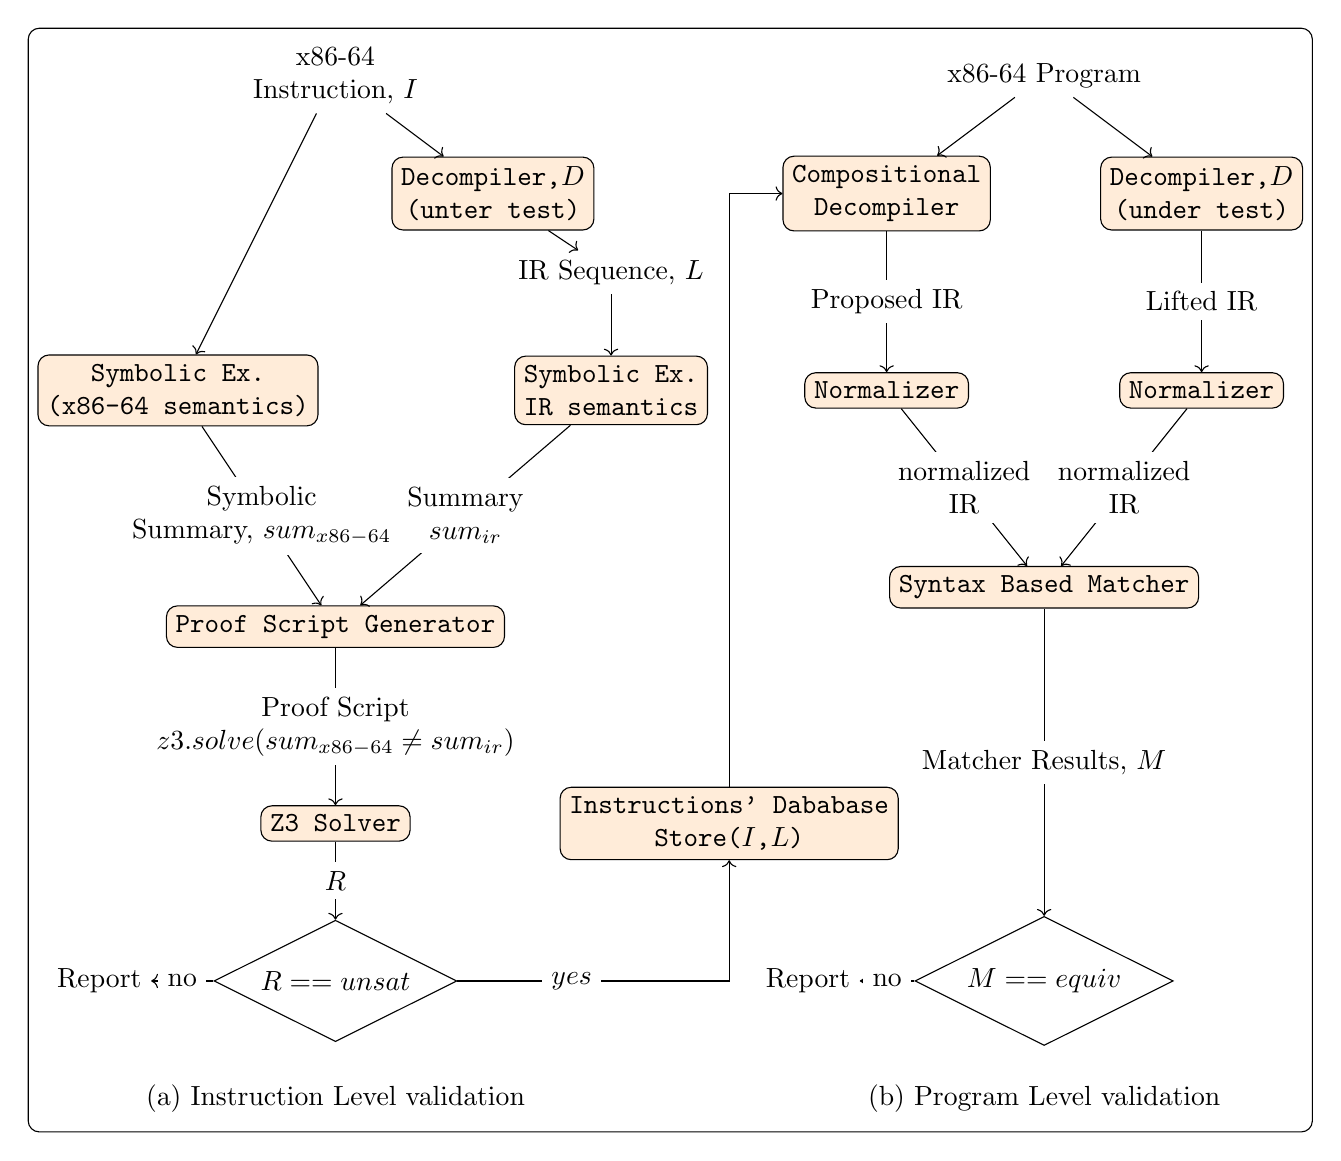
\begin{tikzpicture}[%node distance=2.5cm,
every node/.style={fill=white}, align=center]
\tikzset{%
    %>={Latex[width=2mm,length=2mm]},
    % Specifications for style of nodes:
    base/.style = {rectangle, rounded corners,
         text centered},
    process/.style = {base,  fill=orange!15, font=\ttfamily, draw=black},
    basic box/.style = {
        shape = rectangle,
        align = center,
        draw  = #1,
        %fill  = #1!25,
        rounded corners},
      header node/.style = {
        %Minimum Width = header nodes,
        font          = \strut\Large\ttfamily,
        text depth    = +0pt,
        fill          = white,
        draw},
      header/.style = {%
        inner ysep = +1.5em,
        append after command = {
            \pgfextra{\let\TikZlastnode\tikzlastnode}
            node [header node] (header-\TikZlastnode) at (\TikZlastnode.north) {#1}
            %node [span = (\TikZlastnode)(header-\TikZlastnode)] at (fit bounding box) (h-\TikZlastnode) {}
        }
      },
}
\def\blockhdist{2cm}
\def\blockvdist{1.5cm}
\def\phasehdist{8cm}


%%%%%%%%%%%%%%% PHASE I
\node (instr)          [base]  {\ISA\\ Instruction, $I$};
\node (SIVmcsema)   [process, below of=instr, yshift=-0.5cm, xshift=\blockhdist]  {Decompiler,$D$\\(unter test)};
\node (irseq)          [base,below of=SIVmcsema, xshift=\blockvdist]  {IR Sequence, $L$};
\node (instrSymEx)   [process, below of=instr, yshift=-2*\blockvdist, xshift=-\blockhdist] {Symbolic Ex.\\(\ISA semantics) };
\node (irSymEx)   [process, below of=irseq, yshift=-0.5cm] {Symbolic Ex.\\IR semantics};
\node (proofGen)   [process, below of=instr, yshift=-4*\blockvdist] {Proof Script Generator};
\node (solver)   [process, below of=proofGen, yshift=-\blockvdist] {Z3 Solver};
\node (decide1)     [draw, below of=solver, yshift=-1cm, diamond, aspect=2]  {$R == unsat$};
\node (report1)       [left of=decide1, xshift=-\phasehdist/4]  {Report};
\node (caption1)     [below of=solver, yshift=-2.5cm] {(a) Instruction Level validation};

\draw[->]             (instr) -- (SIVmcsema);
\draw[->]             (SIVmcsema) -- (irseq);
\draw[->]     (instr) -- (instrSymEx);
\draw[->]     (irseq) -- (irSymEx);
\draw[->]     (instrSymEx) -- node {Symbolic\\Summary, $sum_{\ISA}$} (proofGen);
\draw[->]     (irSymEx) -- node {Summary\\$sum_{ir}$ } (proofGen);
\draw[->]     (proofGen) -- node {Proof Script\\$z3.solve(sum_{\ISA} \ne sum_{ir})$} (solver);
\draw[->]     (solver.south) -- node {$R$} (decide1.north);
\draw[->]     (decide1.west) -- node {no} (report1);

%%%%%% Store
\node (store)     [process, right of=solver, xshift=\phasehdist/2]{Instructions' Dababase\\Store({$I$,$L$})};
\draw[->]       (decide1.east) -| node[xshift=-2cm] {$yes$} (store.south);


%%%%%%%%%%%% PHASE II
\node (start)             [base,right of=instr, xshift=\phasehdist]                       {\ISA Program};
\node (compd)             [process, below of=start, yshift=-0.5cm, xshift=-\blockhdist]          {Compositional\\Decompiler};
\node (mcsema)             [process, below of=start, yshift=-0.5cm, xshift=\blockhdist]          {Decompiler,$D$\\(under test)};
\node (normalizer1)             [process, below of=compd, yshift=-\blockvdist]   {Normalizer};
\node (normalizer2)         [process, below of=mcsema, yshift=-\blockvdist]   {Normalizer};
\node (matcher)     [process, below of=normalizer2, yshift=-\blockvdist, xshift=-\blockhdist]   {Syntax Based Matcher};
\node (decide2)     at (decide1 -| matcher) [draw,  diamond, aspect=2]  {$M == equiv$};
\node (caption2)     at (caption1 -| matcher) {(b) Program Level validation};
\node (report2)       [left of=decide2, xshift=-\phasehdist/4]  {Report};
 
 
\draw[->]             (start) -- (compd);
\draw[->]             (start) -- (mcsema);
\draw[->]     (compd) -- node {Proposed IR} (normalizer1);
\draw[->]     (mcsema) -- node {Lifted IR} (normalizer2);
\draw[->]     (normalizer1) -- node {normalized\\IR} (matcher);
\draw[->]     (normalizer2) -- node {normalized\\IR} (matcher);
\draw[->]     (matcher) -- node {Matcher Results, $M$} (decide2);
\draw[->]     (store.north) |-  (compd.west);
\draw[->]     (decide2.west) -- node {no} (report2);

%% Outter box
\begin{scope}[on background layer]
\node[fit = (compd)(mcsema)(start)(matcher), basic box = black,] (Phase1) {};
    \node[fit = (compd)(mcsema)(start)(matcher)(instr)(solver)(irseq)(instrSymEx)(irSymEx)(caption1)(caption2), basic box = black,] (Overview) {};
\end{scope}

\end{tikzpicture}


\end{figure*}



\section{Single \ISA Instruction Validation}
\section{Preliminaries}
\label{sec:Prelim}

Here we provide background on the \K framework and the \Strata project~\cite{Heule2016a} (used for our baseline semantics).

% briefly explain pieces of \ISA ISA necessary for our
% presentation. We also talk about \K, a semantics engineering tool which we
% chose to formalize our semantics into and  \Strata which gives us a head-start towards modeling the semantics of \ISA instructions.

%%% (VSA) DISABLE X86 BACKGROUND: IT IS WIDELY KNOWN
%\subsection{\ISA Instruction Set Architecture}

\ISA is the 64-bit extension of x86, a family of backward-compatible ISAs.
% x64 is a generic name for the 64-bit extensions to Intel's and AMD's 32-bit x86 instruction set architecture (ISA). 
%
We briefly explain some details of the architecture.

% Registers:
\ISA has the sixteen 64-bit general purpose registers (\reg{rax}--\reg{rdx}, \reg{rsi}, \reg{rdi}, \reg{rsp}, \reg{rbp}, \reg{r8}--\reg{r15}), and the two $64$-bit special registers (\reg{rip} and \reg{rflags}).
The lower $32$-, $16$- and $8$-bit portions of the register are referenced by the sub-register variants, e.g., \reg{eax}, \reg{ax}, and \reg{al} for \reg{rax}, respectively.
% \cmt{All these registers are used for storing integer values.}
The Haswell \ISA ISA additionally has sixteen 256-bit SIMD registers (\reg{ymm0}--\reg{ymm15}) along with the lower 128-bit sub-register variants (\reg{xmm0}--\reg{xmm15}).
% \cmt{, which are used for floating-point and packed operations.}

The \reg{rflags} register stores the current state of the processor.
Specifically, for example, the status flags such as the carry flag (\s{cf}), the parity flag (\s{pf}), the adjust flag (\s{af}), the zero flag (\s{zf}), and the sign flag (\s{sf}) are stored in \reg{rflags}.
These status flags are set according to the result of arithmetic and logical instructions.
% the status flags used mostly in user-level \ISA programs, and updated by arithmetic-logical instructions according to the result of the operation.
Some of control transfer instructions are performed based on the values of these flags.

% Addressing modes: 
\ISA supports the addressing modes, expressions that calculate a memory address to be read or written to. The addressing modes are used as the source or the destination of instructions that access the memory.
The addressing mode expressions can be generalized as:
$\s{base} + \s{index} \times \s{stride} + \s{offset}$.
In the assembly code, for example, \instr{-4(\reg{rax}, \reg{rbx}, 8)} denotes the address mode ``$\reg{rax} + \reg{rbx} \times 8 - 4$''.

% \cmt{      
% \begin{lstlisting}[style=SIMPRULES]
%     D (%RB, %RI, S)
%         RB is register for base
%         RI is register for index (0 if empty)
%         D is displacement (0 if empty)
%         S is scale 1, 2, 4 or 8 (1 if empty)
%     Effective Address: Mem[%RB + D + S*%RI]
% \end{lstlisting}
% }   

% Instruction variants:
% If an instruction access memory, we call it memory instruction. Else, if the instruction takes constant, then it is called immediate instruction. Otherwise, it is a register instructions.
\ISA has three types of instructions depending on the types of their operands: register instructions (with only register operands), memory instructions (with address mode operands), and immediate instructions (with constant operands).
The same mnemonic can be used for the different types of instructions.
For example, the mnemonic \instr{add} can be used for the register instructions (e.g., \instr{addq \reg{rax}, \reg{rbx}}\footnote{Throughout the presentation we will be using the {AT\&T} assembly syntax~\cite{Syntax} where the destination operand comes after source operands.}), the memory instructions (e.g., \instr{addq -4(\reg{rax}), \reg{rbx}}), and the immediate instructions (e.g., \instr{addq \$1, \reg{rbx}}).
% Throughout this paper, we will count each type of instructions as a different instruction.
% In the presentation, we will count them as different insructions ( and call them  instructions variants). Also different opcodes in the Intel manual are counted separately towards total instruction count. 
% \cmt{Whereas, register instructions differing on register names, immediate instructions differing on  constant values and memory instructions   differing on  memory addresses will be counted once towards total instruction count. }




\subsection{K Framework}\label{sec:KF}

%\K~\cite{k-primer-2013-v32} \cmt{\url{http://kframework.org}} is a framework for
%defining formal language semantics. Given a syntax and a semantics of a language, \K
%generates a parser, an interpreter, as well as formal analysis tools such as
%model checkers and deductive program verifiers, at no additional cost. Using
%the interpreter, one can test their semantics immediately, which significantly
%increases the efficiency of semantics developments. Furthermore, the formal
%analysis tools facilitate formal reasoning about the given language semantics.
%This helps both in terms of applicability of the semantics and in terms of
%engineering the semantics itself.
%
%We   refer the reader to~\cite{k-primer-2013-v32, rosu-serbanuta-2010-jlap} for
% details. In a nutshell, in \K, a language syntax is given using conventional
%Backus-Naur Form (BNF). A language semantics is given as a parametric
%transition system, specifically a set of reduction rules over configurations. A configuration is an algebraic representation of the
%program code and state. Intuitively, it is a tuple whose elements
%(called cells) are labeled and possibly nested. Each cell represents a
%semantic component, such as the memory or the registers. A special cell, named \s{k}, contains a
%list of computations to be executed. A computation is essentially
%a program fragment, while the original program is flattened into a
%sequence of computations. A rule describes a one-step transition
%between configurations, giving semantics to language
%constructs. Rules are modular; they mention only relevant cells that
%are needed in each rule, making many rules far more concise and easy to read
%than in some other formalisms.



% One of the most appealing aspects of K is its modularity. It is very rarely the
% case that one needs to touch existing rules in order to add a new feature to
% the language. This is achieved by structuring the configuration as nested cells
% and by requiring the language designer to mention only the cells that are
% needed in each rule, and only the needed portions of those cells. For example,
% the above rule only refers to the \s{k} and \s{regstate} cells, while
% the entire configuration contains many more cells (Figure
% ~\ref{fig:config}). This modularity makes for compact and human
% readable semantics, and also helps with the overall effectiveness of the
% semantics development. For example, even if new cells are later added to
% configuration, to support new features, the above rule does not change.

% \input{figures/configuration.tex}

\subsection{Strata Project}\label{sec:prelimstrata}
%% Support Count 
\Strata~\cite{Heule2016a} automatically synthesized formal semantics of \strataWithDupIS{} instruction variants (representing \strataIntel{} unique mnemonics) of the \ISA Haswell ISA. 
%% Set of test input 
The algorithm to learn the formal semantics of an instruction, say \s{IS}, starts with a small set of instructions, called base set \s{B}, whose semantics are known and trusted; a set of test inputs \s{T}, and the output behavior of \s{IS} obtained by executing \s{IS} on \s{T}. Then \Stoke~\cite{Stoke2013} is used  to synthesize  instruction sequences which contain instructions from \s{B} and match the behavior of \s{IS} for all test cases in \s{T}. Given two such generated instruction sequences \s{IS} and \s{IS}$^\prime$, their equivalence is decided  using an SMT solver and the trusted and known  semantics from the base set. If the two sequences are
semantically distinct, then the model produced by the SMT solver is used  to obtain
an input \s{t} that distinguishes \s{IS} and \s{IS}$^\prime$, and \s{t} is added to \s{T}. This process of synthesizing instruction sequence candidates and accepting or rejecting them based on equivalence checking with previous candidates, is repeated until a threshold is reached, which in their implementation is based on the number of accepted instruction sequences. 

%% Generalization 
\cmt{
Using the above technique, they first came up with the semantics of $692$ register
and $120$ immediate instructions. Then they used ``generalization'' of the register
instructions to get a total support count of \strataWithDupIS. Generalization is based on their hypothesis that the memory or immediate variants will behave identically with corresponding register variant (other than where the inputs come from) and hence can use the same formula as register variants. They validate this hypothesis using random testing. }

%% Two format of output
For each instruction, \Strata manifested its semantics in terms of two related artifacts.
The first artifact is an instruction sequence and the second is a set of SMT formulas 
in the bit-vector theory, one for each output register. 
The second is obtained by symbolically executing the first.

\cmt{
\Stoke~\cite{Stoke2013} contains manually written specifications  for a subset of the
x86-64 instruction set and there are APIs to generate SMT formulas from those specifications. 
\Strata uses those formulas to compare against the ones learned
by stratification by asking an SMT solver if the formulas are equivalent. For
example, for the instruction \instr{andnq \%rdx, \%rcx, \%rbx} the manually
written specification looks like the following:

\begin{lstlisting}[style=C++, label={lst:CS5}, caption={Manually Writen  specification for \instr{andnq
\%rdx, \%rcx, \%rbx}}]
semantic_function (
  Operand dst, Operand src1, Operand src2, 
  // dst == %rbx, src1 == %rcx, src2 == %rbx
  SymBitVector a, SymBitVector b, SymBitVector c, 
  // a, b, c are symbolic values for dst, src1, 
  // src2 resp. 
            SymState& ss) {
  // The symbolic state to be updated with the 
  // behaviour of the instruction     
  auto tmp = (!b) & c;
  
  // Setting destinaton
  ss.set(dst, tmp); 
  // Setting of, cf to false 
  ss.set(eflags_of, SymBool::_false()); 
  ss.set(eflags_cf, SymBool::_false());
  // Updating sf, zf based on result
  ss.set(eflags_sf, tmp[dst.size()-1]);
  ss.set(eflags_zf, tmp == SymBitVector::constant(dst.size(), 0));
  // Setting af, pf to undefined values
  ss.set(eflags_af, SymBool::tmp_var());
  ss.set(eflags_pf, SymBool::tmp_var());
}
\end{lstlisting}
}

\subsection{McSema}\label{sec:McS}



\section{\ISA Program-Level Validation}
\subsection{Compositional Decompiler}
\subsection{Normalizer}
\subsection{Matcher}

%\section{Formalization of \ISA Semantics}
\label{sec:harvestsema}
This section presents how we get the complete semantics of all the
user-level instructions. Section~\ref{sec:IC} details the scope of our work. Section~\ref{sec:Approach} mentions how we leverage the information available in \Strata, our baseline semantics. Section~\ref{sec:x86sema} explains how we formalize our model in \K.

\subsection{Scope of the Work}\label{sec:IC}
\SC{We support all but a few non-deprecated user-level instructions. The support includes  \currentIS{} total variants of the Haswell \ISA ISA (representing \currentIntel{} out of \totalIntel{} 
unique mnemonics)}. The entire implementation took 8 man-months, with the lead author having prior experience in binary decompilation and strong familiarity with the \ISA architecture and documentation.
% (not including extensive time spent on projects related to binary decompilation that gave the lead author relevant experience and strong familiarity with the \ISA architecture and documentation).  
Below is a summary of the instruction categories that we support.
%\begin{itemize}
%    \item \textbf{General-Purpose Instructions:} These implement data-movement, arithmetic, logic, control-flow, string operations (including repeated- and fast- string operations).
%    
%    \item \textbf{Streaming SIMD Extensions (SSE) Instructions \&   subsequent extensions (SSE-2, SSE-3, SSE-4.1, SSE-4.2):} Instructions in this category operate on integer, string or floating-point values stored in $128$-bit xmm registers. Among other things, the category features instructions related to conversions between integer and floating-point values with selectable rounding mode, and string processing.
%    
%    \item \textbf{Advanced Vector Extensions (or AVX) \& subsequent extensions (Fused-Multiply-Add (or FMA) \& AVX2):} These instructions operate on integer or floating-point values stored in $256$-bit ymm registers; a majority of which are promoted from SSE instruction sets. Additionally, the category features enhanced functionalities specific to AVX \& AVX2, like  broadcast/permute, vector shift, and non-contiguous data fetch operations on data elements. 
%    \item \textbf{$\textbf{16}$-bit Floating Point Conversion (or F16C):} These instructions implement conversions between single-precision ($32$-bit) and half-precision ($16$-bit) floating-point values. 
%\end{itemize}

\begin{itemize}
\item \emph{General-Purpose:~}
These implement data-movement, arithmetic, logic, control-flow, string operations (including fast- and repeated- string operations).
    
\item \emph{Streaming SIMD Extensions (SSE) \& subsequent extensions (SSE-2, 
SSE-3, SSE-4.1, SSE-4.2):~}
Instructions in this category operate on integer, string or floating-point values stored in $128$-bit xmm registers. Among other things, the category features instructions related to conversions between integer and floating-point values with selectable rounding mode, and string processing.
    
\item \emph{Advanced Vector Extensions (AVX) \& subsequent extensions 
(Fused-Multiply-Add (FMA) \& AVX2):~}
These instructions operate on integer or floating-point values stored in $256$-bit ymm registers; a majority of which are promoted from SSE instruction sets. Additionally, the category features enhanced functionalities specific to AVX \& AVX2, like  broadcast/permute, vector shift, and non-contiguous data fetch operations on data elements. 

\item \emph{16-bit Floating-Point Conversion (or F16C):~}
These instructions implement conversions between single-precision ($32$-bit) and half-precision ($16$-bit) floating-point values. 
\end{itemize}

Instructions which are \emph{not included} in the current scope of work are:
\begin{itemize}
\item System-level instructions, which are related to the operating system, 
protection levels, I/O, cache lines, and other supervisor instructions; 
\item x87 \& MMX instructions, consisting of legacy floating-point and 
vector operations, respectively, which are now superseded by SSE; 
\item Concurrency-related operations, including atomic operations and 
fences; and 
\item Cryptography instructions, which support cryptographic processing 
specified by Advanced Encryption Standard (AES). 
\end{itemize} 
%
\SC{We note that while there is no inherent limitation in supporting the above 
instructions with our approach, the system-level instructions require to 
formulate an abstraction of different architectures and operating systems, 
which is a significant effort that is orthogonal to the presented effort of 
formalizing the user-level instructions.}
%\SC{Note that, there is no inherent limitation in supporting system-level and 
%cryptography instructions with our approach. However, the system-level 
%instructions require to formulate an abstraction of different architectures 
%and 
%operating systems, which is an orthogonal, significant effort that we think 
%should be deserved as an independent work, and we wanted to separate it from 
%the presented effort of formulating the user-level instructions. 
Nevertheless, K framework makes it easy to add additional state components 
without modifying rules for operations that do not require those components. We 
expect our approach to work equally well compared with existing approaches, 
such as ~\cite{Goel:ProCoS17}, which implements a subset of system-level 
instructions. On the other hand, the cryptography instructions are omitted 
mainly because they are not given a high priority.

\subsection{Overview of the Approach}
\label{sec:Approach:Overview}

Briefly, our approach is as follows.
%
We first defined the machine configuration and underlying infrastructure in the \K framework, in order to define, execute and test the \ISA semantics.
%
\SC{To leverage previous work as much as possible, we took the semantic rules of all the instructions supported in Strata, which amounts to about 60\% of the instructions in scope, in the form of SMT formulas.}
%
We corrected, improved or simplified many of the baseline rules.
%
We then translated these SMT formulas from Strata into \K rules using a script, and tested the resulting rules by comparing with the Strata rules using Z3.
%
These steps give us a validated initial set of semantic rules in \K for about 60\% of the target instructions (our ``baseline'' set).

We attempted to extend the stratification approach in Strata to define additional rules automatically, in two ways: (i) augmenting their base set \s{B}, and (ii) constraining the search space manually using knowledge of instruction behaviors.  Both these attempts failed; they worked only for a few instructions, but in general, we found them to be impractical. Specifically, we added $58$ base instructions to the base set, and learned the semantics of $70$ new instructions, which are variants of the added  instructions, in $20$ minutes, but no more even after we kept running for two days. Also, we tried constraining the search space by manually populating it with relevant instructions. The lesson we learned from these experiments is, getting the right set of base instructions or a constrained search space for a complex instruction need an insight about the semantics of that instruction itself. We found that the effort to extract such information from the manual is about the same  as manually defining that instruction.
 

%\Comment{SANDEEP: Please check this last sentence and fix / improve.}

We then manually added \K rules for the remaining 40\% of the target instructions by systematically translating their description of the Intel manual into \K rules, in some cases cross-referencing against semantics available in Stoke.
%
The outcome was a complete formal specification of user-level \ISA in \K.

We validated this semantics in three ways, as described in Section~\ref{sec:Eval}.
%
First, we use the \K interpreter to execute the semantics of \emph{each} instruction for 7,000+ test inputs (each input is a processor state configuration) and compared the output directly with the hardware behavior for the same instruction.
%
Second, we repeated this experiment using the applicable programs in the \SC{GCC C-torture tests~\cite{CTORTURE}}.  % (\TortureInclude{} out of \TortureTotal{} tests).
%
Third, we compared against the semantics defined in the Stoke project for about 330 instructions that were omitted in Strata (thus not included in our baseline), using an SMT solver.

These validation experiments uncovered bugs in the Intel manual, in Strata's simplification rules, and in the Stoke semantics.  All these bugs were reported to the authors, and most have been acknowledged and some have been fixed.  The details are in Section~\ref{sec:Eval}.



%% \section{Defining Semantics of \ISA ISA in K}\label{sec:x86sema}

% This section is about defining the semantics of individual instructions in \K along with  execution environment, which is used to execute instructions using \K framework. \cmt{We describe the different components of our definition and give a number of example of the semantics.}

% \cmt{ \subsection{Syntax}
% Our model parsers the syntax of \ISA assembly language program which is generated either from the source code using GNU assembler~\cite{GNUAS} or
% directly from the binary using disassemblers like Objdump~\cite{Objdump}.  
% }

\subsection{Program Configuration}\label{sec:x86sema}
Defining a language semantics in \K requires defining the program configuration, the semantics of how programs are evaluated (i.e., the execution environment), and the semantics of the statements or instructions.  We begin with the configuration.

\begin{figure}
  \centering
  %
  \renewcommand{\dotCt}[1]{\scriptstyle\s{#1}}
  \newcommand{\regstate}{\scriptstyle\s{ID}_\s{regname} \;\mapsto\; \s{Value}}
  \newcommand{\argc}{\scriptstyle\s{Int}}
  \newcommand{\argv}{\scriptstyle\s{Address}} 
  \newcommand{\entrypoint}{\scriptstyle\s{Address}}
%  \newcommand{\labeladdress}{\scriptstyle\textit{ID}_\textit{Label Name} \;\mapsto\; \textit{Address}}
  \newcommand{\codemem}{\scriptstyle\textit{Address} \;\mapsto\; \textit{Instruction}}
  \newcommand{\datamem}{\scriptstyle\s{Address} \;\mapsto\; \s{Value}}
  \newcommand{\bssmem}{\scriptstyle\textit{Address} \;\mapsto\; \textit{Value}}
  \newcommand{\stackmem}{\scriptstyle\textit{Address} \;\mapsto\; \textit{Value}}
  \newcommand{\heapmem}{\scriptstyle\textit{Address} \;\mapsto\; \textit{Value}}
  %
$
\kall{T}{
  \begin{array}{@{}c@{}}
  \kall{k}{\dotCt{K}} \mathrel{}
  \mathrel{}
  \kall{regstate}{\regstate} \mathrel{}
  \mathrel{}
  \kall{memstate} {\datamem} \mathrel{}
  \mathrel{}
  \cdots
  \cmt{ 
  \kall{executionEnv}{ 
  \kall{commandineArgs}{
    \kall{argc}{\argc} \mathrel{}    
    \kall{argv}{\argv} \mathrel{}
  } \mathrel{}
  \kall{entryPoint}{\entrypoint} \mathrel{}
}}
%  \kall{labelAddress}{\labeladdress} \mathrel{}
  \end{array}
}
$
  %
\vspace{-10pt}
  \caption{Program Configuration}
  \label{fig:config}
\end{figure}


The \K configuration of a running \ISA program is shown in Figure~\ref{fig:config}. The cells are represented using angle brackets. The outer $\top$ cell contains the cells used during program evaluation.
%\SC{While this figure only shows $3$ cells used mostly during the presentation of our semantics, we use over $60$ in the full semantics.}
The inner \s{k} cell contains a list of computations to be executed. \SC{Below we describe the two other inner cells.}\footnote{%
\SC{We omit other auxiliary cells (marked by ``$\cdots$'') for the simplicity of the presentation.}
}

\emph{Register State.~}
The \s{regstate} cell contains a  map from registers or flag names to values. \SC{Note that, all the values or addresses, stored in registers, memory (described next) or flags, are represented as bit-vectors which are depicted as \bv{W}{V}, and interpreted as a bit-vector of size \s{W} and value \s{V}.} The register names include the sixteen general purpose registers, \reg{rip}, and the sixteen SIMD registers.  The value mapped to a register name is a $64$-width bit-vector (or a $256$-width one for the SIMD registers). Values for sub-register variants are derived from the register values by extracting the relevant bits. \cmt{In the \s{regstate} map, }We store individual flag names (mapped to a bit-vector value of width $1$) as opposed to a $64$-bit \s{rflags} register. Every access (read/write) of \reg{rflags} retrieves the entries in the \s{regstate} map for the individual flags.

\emph{Memory State.~}
Our memory model is inspired by previous efforts ~\cite{TSL:TOPLAS13, Ellison}.
The \s{memstate} cell is a map from $64$-bit addresses to bytes, which specifies the \SC{byte-addressable memory}\footnote{\SC{Byte-addressability allows the model to specify both aligned and unaligned accesses in the same principle.}}, but our implementation is flexible enough to use alternative memory  representations with addressing of $2$-byte or $4$-byte quantities.  Our memory layout is ``flat'', in which all available memory locations can be addressed, but we do have logical partitions\footnote{These abstractions are useful for executing \ISA programs.} of the memory into sections like code, data and stack.  The following is an example snapshot of a memory state,  holding a $4$-bytes integer value $65535$:
\begin{tightcenter}
    \small
    \newcommand{\bytecell}[2]{\s{byte}({#1},\;\;{#2})}
    $
    \kall{memstate} {
        \begin{array}{c}
        %\begin{array}{ll}
        4 \;\mapsto\;  \bytecell{0}{32'65535} \quad
        5 \;\mapsto\;  \bytecell{1}{32'65535}\\
        6 \;\mapsto\;  \bytecell{2}{32'65535} \quad
        7 \;\mapsto\;  \bytecell{3}{32'65535}\\
        \end{array}
    }
    $
\end{tightcenter}
\SC{Here the memory address $4$ stores the $0^\text{th}$ byte of the bit-vector \bv{32}{65535}, the address 5 stores the $1^\text{st}$ byte, and so on}. When memory is read, requested bytes are aggregated according to the size of the memory access.



\subsection{Semantics of Execution Environment}
%\begin{figure*}[t]
\begin{tabular}{l}      
\begin{lstlisting}[basicstyle=\scriptsize,morekeywords={andBool, requires, ensures, and, rule},keywordstyle=\color{blue},escapeinside={(*}{*)},]
rule <k>  (OpC:Opcode OpR:Operands):Instruction) Rest:Instructions ~> fetch </k>
\end{lstlisting} \\

\begin{lstlisting}[basicstyle=\scriptsize,morekeywords={andBool, requires, ensures, and, rule},keywordstyle=\color{blue},escapeinside={(*}{*)},]
rule  <k> OpC:Opcode OpR:Operands => (*\textbf{.}*) ...</k>
   <memstate>... L <- storedInstr(OpC OpR) ...</memstate>
   <nextLocPc> L:Address => L + sizeofInstr(OpC OpR) </nextLocPc>
\end{lstlisting} \\

\begin{lstlisting}[basicstyle=\scriptsize,morekeywords={andBool, requires, ensures, and, rule},keywordstyle=\color{blue},escapeinside={(*}{*)},]
rule <k> fetch => execinstr(OpC OpR) ~> fetch ... </k>
  <memstate>... L |-> storedInstr(OpC OpR) ...</memstate>
  <regstate>... "RIP" |-> ( L => sizeofInstr(OpC OpR))  ...</regstate>
\end{lstlisting} \\

\begin{lstlisting}[basicstyle=\scriptsize,morekeywords={andBool, requires, ensures, and, rule},keywordstyle=\color{blue},escapeinside={(*}{*)}]
rule <k> fetch => (*\textbf{.}*)  ... </k>
  <memstate> codeMap:Map  </memstate>
  <regstate> "RIP" |-> BV(*$_\s{rip}$*) </regstate>
    requires not iloc( {RSMap["RIP"]}:>MInt ) in_keys ( CMap )
\end{lstlisting} \\


\end{tabular}
        \caption{Semantics of Execution Environment}
        \label{fig:compSema}
\end{figure*}


\cmt{\begin{figure*}[t]

$
\begin{array}{@{}l@{}}

\mbox{\scshape {\scriptsize rule}: \textbf{\scriptsize inital value of k cell}} \\
\kall{k}{\scriptsize {\tt initEnv}(\$ARGV)\kra ((OpC{\tt:Opcode}\;\; OpR{\tt:Operands}){\tt:Instruction} \;\;Rest{\tt:Instructions})\kra{\tt fetch}} \\
\multicolumn{1}{c}{(a)} 
\\[0.3cm]

\mbox{\scshape {\scriptsize rule}: \textbf{\scriptsize load instruction}} \\
\kall{k}{\scriptsize \reduce{OpC{\tt:Opcode}\;\; OpR{\tt:Operands}}{\cdot} \ellipses}
\mathrel{}
\kall{memstate}{\scriptsize \ellipses \reduce{\cdot}{BV_{L} \;\mapsto\; (OpC\;\;OpR)} \ellipses}
\mathrel{}
\kall{nextloc}{\scriptsize  \reduce{BV_{L}}{BV_{L} + {\tt sizeof}(OpC\;\;OpR)}}
\\
\multicolumn{1}{c}{(b)} 
\\[0.3cm]

\mbox{\scshape {\scriptsize rule}: \textbf{\scriptsize fetch instruction}} \\
\kall{k}{\scriptsize \reduce{{\tt fetch}}{{\tt exec}(OpC\;\;OpR) \kra fetch} \ellipses}
\mathrel{}
\kall{memtate}{\scriptsize \ellipses BV_{L} \;\mapsto\; (OpC\;\;OpR) \ellipses}
\mathrel{}
\kall{regstate}{\scriptsize \ellipses RIP \;\mapsto\; \reduce{BV_{L}}{BV_{L} + {\tt sizeof}(OpC\;\;OpR)} \ellipses}
\\
\multicolumn{1}{c}{(c)} 
\\[0.3cm]

\mbox{\scshape {\scriptsize rule}: \textbf{\scriptsize program termination}} \\
\kall{k}{\scriptsize \reduce{{\tt fetch}}{\cdot} \ellipses}
\mathrel{}
\kall{memstate}{\scriptsize codeMap{\tt :Map}}
\mathrel{}
\kall{regstate}{\scriptsize \ellipses RIP \;\mapsto\; BV_{rip}\ellipses}
\\
  \qquad \texttt{when notBool}\;\;BV_{rip}\;\; \texttt{in\_keys}\;\;codeMap 
  \mathrel{}
\\
\multicolumn{1}{c}{(d)} 
\\
\hline
\end{array}
$

%
\caption{Semantics of Execution Environment}
\label{fig:compSema}
\end{figure*}
}


We now give the reader a flavor of our semantics, by discussing a few of the roughly $5,200$ rules\footnote{Each rule is 17 LOC on average, and the total size is 15 KB of text.} that we defined to model the entire semantics.
%\Comment{Can you list how many of these rules came from Strata unchanged, 
%how many had to be "fixed" in various ways, how many you wrote yourself?}
We first explain the semantics of the execution environment, which involves all the machinery used for executing \ISA programs.
We will explain the semantics of individual instructions in the next section.

\SC{The execution of an \ISA program begins with initialization of the configuration with the following contents of the \s{k} cell. }
\begin{lstlisting}[style=KRULE]
           <k> $PGM:Instructions (*$\kra$*) fetch </k>
\end{lstlisting}
\SC{The symbol $\kra$ is used to separate the computations in the \s{k} cell and ``\s{:T}'' to represent the type of a term.}


Concisely, the semantics of execution of an \ISA program involves initializing the memory by reading the program instructions (\s{\$PGM}), from the \s{k} cell, one at a time until all the instructions are loaded in memory. The memory-loaded instructions are then fetched one at a time, using the \s{fetch} computation, to get executed. The instruction to be executed next is pointed to by the instruction pointer register \reg{rip}.  

Next, we describe the rule applied to initialize memory with instructions one at a time.
\begin{lstlisting}[style=KRULE]
rule  <k> OpC:Mnemonic OpR:Operands (*$\Rightarrow$*) (*\textbf{.}*) ...</k>
 <memstate> M:Map (*$\Rightarrow$*) M[L (*$\leftarrow$*) (OpC OpR)] </memstate>
 <nextloc> L:Address (*$\Rightarrow$*) L + instrSize(OpC OpR) </nextloc>
\end{lstlisting}
The \s{k} cell contains the instruction to be processed next.  \s{Mnemonic} and \s{Operands} denote the types of the terms used to represent an instruction.  The `$\Rightarrow$' symbol
represents a reduction (i.e., a transition relation). A cell without the `$\Rightarrow$' symbol means that it is read but not changed by the rule. \K allows us to use ``.'' to represent an empty computation and ``...'' to match the portions of a cell that are neither read nor written by the rule. The above rule essentially  stores each instruction in memory, which is modeled as a map, at an address \s{L} given by the %\s{nextloc}\textsuperscript{\ref{nextloc}} cell. Subsequently, 
\SC{\s{nextloc}}\footnote{\label{nextloc}\SC{The \s{nextloc} cell is a auxiliary cell that holds the next memory location to store an instruction, which we omit in the program configuration (Figure~\ref{fig:config}) for the sake of simplicity.}} cell. Subsequently,
the \s{nextloc} cell gets updated to an appropriate address  used for storing the next instruction.  Once the entire program is loaded, the fetch-and-execute cycle starts, which is realized by the following rule:
\begin{lstlisting}[style=KRULE]
rule <k> fetch (*$\Rightarrow$*) exec(OpC OpR) (*$\kra$*) fetch ... </k>
  <memstate>... L (*$\mapsto$*) (OpC OpR) ...</memstate>
  <regstate>... 
    "RIP" (*$\mapsto$*) ( L (*$\Rightarrow$*) L + instrSize(OpC OpR))  
  ...</regstate>
\end{lstlisting}
%\Comment{It is not clear what kind of term \Code{exec(OpC OpR)} is: is it a special function defined somewhere, or a separate rule? I'm not familiar enough with K, but remember that reviewers won't be familiar either!}
%
 The rule above says that if the next thing to be evaluated is a fetch computation 
 (referred in the rule as \s{fetch}), then one should match \reg{rip} in the environment 
 to find its value \s{L}
 in \s{regstate}, where \m{L} is matched in \s{memstate} to find the mapped instruction.
 The mapped instruction is then put at the head of the \s{k} cell to be computed next, using a rule \s{exec} for execution (defined later), along with the \s{fetch} computation to be executed in order. The rule also updates the value of \reg{rip} to point to the following instruction. The execution will be terminated when there is no instruction stored in the memory at the address pointed to by \reg{rip}.\footnote{While initializing the stack section of memory, we store an invalid address just before the entry-point function as return address. When the entry point function returned, the invalid return address is popped out of the stack and stored in \reg{rip} leading to program termination.} 

\subsection{Semantics of Individual Instructions}
\label{sec:semantics-of-individual-instructions}

Here we explain how we define the semantics of an instruction in \K using a running example of logical-and-not \instr{andnq -4(\%rsp), \%rbx, \%rax}, which performs a bitwise logical AND of inverted source register operand (\reg{rbx}) with the source memory operand (\mem{-4}{rsp}) and writes the result to destination register \reg{rax}. Additionally the instruction affects all the $6$ status flags (\reg{sf}, \reg{zf}, \reg{of}, \reg{cf}, \reg{af} and \reg{pf}).


%\begin{figure*}[]
    \begin{tabular}{ll} 
        $
       \begin{array}{@{}l@{}}
          \kprefix{k}{\reduce{{\tt exec(pushw\;\;4(\%rsp)\;\;.List)}}
              {{\tt 4(\%rsp)} \kra {\tt exec(pushw\;\;\Box\;\;.List)}}} \mathrel{}
          \mathrel{}  
          \\
           \multicolumn{1}{c}{(a)} 
       \end{array}   
       $               
        & 
       $
        \begin{array}{@{}l@{}}
           \kprefix{k}{\reduce{{\tt 4(\%rsp)}}{{\tt memOffset( BV_{rsp} + 64'4)}}} \mathrel{}
        \kall{regstate}{\ellipses{\tt RSP}\mapsto {\tt BV_{rsp}}\ellipses} \mathrel{} \mathrel{}
       \\
       \multicolumn{1}{c}{(b)} 
       \end{array}  
       $ \\   \\ [1pt]
 
 $
 \begin{array}{@{}l@{}}
  \kprefix{k}{\reduce{
          {\tt memOffset(O)} \kra {\tt exec(pushw\;\;\Box\;\;.List)}}
      { {\tt exec(pushw\;\;memOffset(O)\;\;.List)}}} \mathrel{} 
 \\
 \multicolumn{1}{c}{(c)} 
 \end{array}   
 $               
 & 
 $
 \begin{array}{@{}l@{}}
 \kprefix{k}{\reduce{
         {\tt exec(pushw\;\;memOffset(O)\;\;.List)}}
     { {\tt readFromMem(O, 16) \kra exec(pushw\;\;memOffset(O)\;\;.List)}}} \mathrel{} 
 \\
 \multicolumn{1}{c}{(d)} 
 \end{array}  
 $ \\ \\ 

     
  \multicolumn{2}{c}{
  $
  \begin{array}{@{}l@{}}
  \kprefix{k}{\reduce{
          {{\tt {memValue(V) \kra exec(pushw\;\;memOffset(O)\;\;.List)}}}
      }
      {{\tt storeToMem(V,\;\;getRegisterVal(\%rsp) - 64'2,\;\;16)}}} \mathrel{} 
  \kall{regstate}{\ellipses{\tt RSP}\mapsto \reduce{{\tt BV_{rsp}}}{{\tt BV_{rsp}} - 64'2}\ellipses} \mathrel{} \mathrel{}
  \\
  \multicolumn{1}{c}{(e)} 
  \end{array}
  $      
    }\\ \hline
    \end{tabular}
    \caption{Semantics of \s{pushw (\%rsp)}}
    \label{fig:pushw}
\end{figure*}
















The semantics of most of the instructions can be modeled broadly in $3$ phases: (1) read the data from source operand(s), which could be a register, memory or constant value; (2) operate on the data based on the mnemonic; and (3) write the result(s) to destination operand(s), which could be a register or memory. An instruction may exercise some or all of the above phases. 
   
%\vspace{-2pt}
\paragraph{Read from Source Operand(s)}

Instruction in the running example reads from  register (\reg{rbx}) and memory (\mem{-4}{rsp}) operands. A read from register is modeled as a lookup with register name in the \s{regstate} map and subsequent read of the mapped value or,
for a sub-register, a portion of it. The semantics of register read can be defined as:  
\begin{lstlisting}[style=KRULE]
rule <k> getRegisterVal(R:R64) (*$\Rightarrow$*) BV(*$_\s{r}$*) ...</k>
  <regstate>... R (*$\mapsto$*) BV(*$_\s{r}$*) ...</regstate>
\end{lstlisting}
 In the context of the running example, this rule
is applied when the current computation (at top of the \m{k} cell) is a $64$-bit register
lookup, appeared as  \m{getRegisterVal(\reg{rbx})}, and \m{regstate} contains a register
with name ``\m{RBX}''. This rule resolves the register lookup  to the mapped bit-vector value \m{BV$_r$} (or \m{BV$_\m{RBX}$} for the running example). 

A read from memory involves computing the effective address in the memory, looking-up that address in memory, and reading requested bytes from memory if the memory access is within allowed range.
The following rule is applied to compute the effective address:
\begin{lstlisting}[style=KRULE]
rule <k> 
 (Offset:Int (R:R64)):Mem (*$\Rightarrow$*) ( 64'Offset + BV(*$_\s{r}$*)):Address
...</k>
  <regstate> ... R (*$\mapsto$*) BV(*$_\s{r}$*) ... </regstate>
\end{lstlisting}
\SC{The term to the left of $\Rightarrow$ shows the memory addressing expression, of type \s{Mem}, at the 
top of \s{k} cell, which gets reduced to an effective memory address (or EA).} The EA for the memory operand used in the running example is (64'-4 + \s{BV$_\s{rsp}$}) and is used to do memory read access. The rule for memory read access is responsible to read a memory value of requested number of bits ($64$-bits for the current example) starting from the EA. 
 
%\vspace{-2pt}
\paragraph{Operate on Data}

The rules for operating on operands will be different for each instruction based on the mnemonic. For example, the mnemonic \instr{andnq} requires logical-and-not operation to be computed on the operands.

%\vspace{-2pt}
\paragraph{Write to Destination Operand(s)}

The example instruction writes the result to a destination register \reg{rax}. Also, the flags \s{sf} and \s{zf} are updated based on the result; \s{of} and \s{cf}  are cleared, and \s{af} and \s{pf} are undefined. The rule shown in Figure~\ref{fig:andn-semantics} realizes the destination write operation, where \s{memVal$_{64}$} and \s{BV$_\s{r}$} represents the $64$-bit data values evaluated using the respective rules for reading register and memory operands (mentioned above).
%
%\Comment{Should "R" be "Dest" below in the first regstate rule?}
%
\begin{figure}
\begin{lstlisting}[style=KRULE]
rule <k>
  exec(andnq memVal(*$_{64}$*), BV(*$_\s{r}$*), R:R64) (*$\Rightarrow$*) (*\textbf{.}*)
...</k>
  <regstate>
    "R"  (*$\mapsto$*) _ (*$\Rightarrow$*) ((*$\sim$*)BV(*$_\s{r}$*) & MemVal(*$_{64}$*))
    "SF" (*$\mapsto$*) ((*$\sim$*)BV(*$_\s{r}$*) & MemVal(*$_{64}$*))[63:63]
    "ZF" (*$\mapsto$*) ((*$\sim$*)BV(*$_\s{r}$*) & MemVal(*$_{64}$*)) (*$=$*) 64'0 ? 1'1:1'0
    "OF" (*$\mapsto$*) 1'0
    "CF" (*$\mapsto$*) 1'0
    "AF" (*$\mapsto$*) undef // af and
    "PF" (*$\mapsto$*) undef // pf are undefined.
  ...</regstate>  
\end{lstlisting}
%\vspace{-5pt}
\caption{Example instruction semantics of \instr{andn}}
%\vspace*{-12pt}
\label{fig:andn-semantics}
\end{figure}
The operator ``[i:j]'' extracts bits i down to j from a bit-vector of size n, yielding another  bit-vector of size i - j + 1, assuming that n $>$ i $\ge$ j $\ge$ 0. The operator ``$\&$'' implements bit-wise ``and'' operation. The rule associated with memory write is similar to that for memory read and is skipped here. 

A \ISA program is modeled as a list of instructions and its semantics is  given by composing the semantics of its constituents.

\subsection{Constructing the \ISA Semantics}
\label{sec:Approach}

% we built our complete semantics on top of the \Strata semantics that we took as our baseline.
%
% As mentioned in section~\ref{sec:prelimstrata}, 

\paragraph{Systematic Translation of \Strata Rules to K}

As mentioned in the introduction, we leverage the \Strata~\cite{Heule2016a} semantics to develop our complete semantics, to minimize the overall effort.
We systematically translated their semantics into \K.
%
Specifically, \Strata offers the semantics of \strataWithDupIS{} instruction variants as SMT formulas specifying the behavior of output registers.
For each instruction, we converted the SMT formulas that \Strata provides to a \K specification using a simple script ($\sim$500 LOC).
The ease of this porting is facilitated by the fact that SMT-LIB expressions 
use s-expression (or "symbolic-expression") notation ~\cite{Steele} which eases 
the parsing effort significantly.

To validate the translation, we generated SMT formulas from the translated \K specifications (using APIs provided by the \K framework), and use the Z3 SMT solver to check their equivalence to the corresponding formulas provided by \Strata.
% In the course of the validation, we found bugs in \Strata's SMT formula extraction module.
%
While translating and validating their semantics, we found various issues that we had to fix to establish our baseline semantics.
%
Below we describe the issues we found in \Strata.%, and how we fixed them  as follows.


%\vspace{-2pt}
\paragraph{Status Flags}

We found that \Strata omitted to specify the \reg{af} flag behaviors, as the flag is not commonly used.
However, we faithfully specified the semantics of all the status flags in the \reg{rflags} register, even if some of them are not commonly used, since they may affect the overall program's behavior in some tricky cases, and we do not want to miss any of such details when formally reasoning about the \ISA programs.

% We had to revise the semantics of $689$\footnoteref{note1} instructions that affect the \reg{af} flag, when we borrow the \Strata semantics as our baseline.




%\vspace{-2pt}
\paragraph{Instruction Variants}

\Strata essentially provides the semantics of the register instructions, assuming that the semantics of the memory and immediate instruction variants can be obtained by generalizing the register instructions\footnote{Generalization is based on a hypothesis that the memory or immediate variants will behave identically, on their operands, with corresponding register variant.}.
However, we found that certain memory instructions cannot be inferred by simply generalizing their corresponding register instructions.
%
For example, for \instr{movsd}, one of the 128-bit SSE instructions, its register variant has quite different semantics from the memory variant.
Below are their pseudo-code semantics:
\cmt{
{
\small
\begin{center}
\begin{tabular}[b]{l}
   // Register Variant: movsd \%xmm1  , \%xmm0 \\ 
   {\tt S1.} XMM0[63:0] $\leftarrow$ XMM1[63:0] \\ 
   {\tt S2.} XMM0[127:64] (Unmodified) \\
   \\
   // Memory Variant: movsd  (\%rax) , \%xmm0 \\
   {\tt S1.} XMM0[63:0] $\leftarrow$ MEM\_ADDR[63:0] \\
   {\tt S2.} XMM0[127:64] $\leftarrow$ 0
\end{tabular}
\end{center}
}
}

\medskip
{    
    \scriptsize
    \begin{tabular}{ll}
        \begin{tabular}[c]{c} 
            Semantics of Register Variant\\ 
            (\instr{movsd \%xmm1  , \%xmm})
        \end{tabular} 
            & 
        \begin{tabular}[c]{c}
            Semantics of Memory Variant\\ 
            (\instr{movsd  (\%rax) , \%xmm0})
        \end{tabular} \\ 
        \midrule 
        {\tt S1.} XMM0[63:0] $\leftarrow$ XMM1[63:0] & {\tt S1.} XMM0[63:0] $\leftarrow$ MEM\_ADDR[63:0] \\
        {\tt S2.} XMM0[127:64] (Unmodified)          & {\tt S2.} XMM0[127:64] $\leftarrow$ 0             \\
        &                                                  
    \end{tabular}
}

\noindent As seen, only the memory instruction clears the higher 64 bits of the destination register, which cannot be inferred from the register instruction behavior that does not touch the higher bits at all.
%
We found that another 128-bit SSE instruction, \instr{movss}, has the same generalization issue.
%
For the other instructions, we obtained the memory and immediate variants by generalizing the register variants, and validated the generalization by co-simulating the inferred semantics against a processor.


%\vspace{-2pt}
\paragraph{Immediate Instruction Variants}

There are 118 immediate instruction variants (over the 8-bit constants) that do not have corresponding register instructions.
For those immediate instructions, Strata provides the instruction semantics for each individual constant, resulting in 30,208 (= $118 \times 256$) \SC{formulae}\footnote{Indeed, Strata explicitly provides only 19,783 formulae by randomly sampling $\sim$168 constants out of 256, in average, for each immediate instruction, assuming that the remaining 10,425 formulae can be inferred.} for the immediate instructions' semantics.
We generalized the set of formulae for each immediate instruction into a single semantic rule.
We validated our generalization by cross-checking the generalized semantics with the original using the SMT solver.

% Moreover, there are $118$ immediate variants with $8$-bit constant value, which
% do not have a corresponding register variant to generalized from. \Strata tries to learn $256$ separate formulas for every possible value of
% the $8$-bit immediate operand. We would like the instruction semantics to be concise and maintainable.  For each of those 
% instructions, we manually write  its semantic in \K and then use APIs provided by \K framework to get the
% corresponding SMT formula. We then compare each of those separate formulas, for a
% constant say \s{c}, with our SMT formula by replacing its symbolic inputs  with
% the constant value \s{c}. Upon successful equivalence check, for all values of
% \s{c}, we accept the manually written semantics. We managed to get a concise
% semantics for all of the $118$ immediate variants. \cmt{Note that, had we used \Strata's  formula with a $k$-bit immediate, \Strata needs 2$^k$ formulas each of which has to be checked, but we have $1$ formula which has to be checked 2$^k$ times, so testing cost is similar but final result is exponentially more concise.}
% %         works for all values of the immediate operand) for those instructions
% %     because that way is more intuitive and easy to maintain.  




% the the semantics of  memory or immediate instruction variants which are obtained from the register variant using ``generalization'' by co-simulating it  against a physical x86 machine.

% While doing that,  we found instructions like \instr{movsd (\%rax), \%xmm0} where the generalization from the corresponding register variant, \instr{movsd \%xmm1, \%xmm0} is not faithful. Followings are their specification as per the Intel manuals.

% Clearly, the memory variant cannot be obtained using generalization of the  corresponding register instruction. Same is true with instruction \instr{movss (\%rax), \%xmm0}.   


%\footnote{Even though \Strata have simplification rules to prevent formula blowup but we found that they are not adequate for many instructions. Hence we added $13$ additional rules.}
 
%\vspace{-2pt}
\paragraph{Formula Simplification}

Due to the nature of the stratification, \Strata provides complex formulae for certain instructions.
%
We simplified those complex formulae by either applying additional $13+$ 
simplification rules (Figure~\ref{fig:simpl-rules} mentions some of those) than what \Strata originally had  or 
manually 
translating into simpler ones.  
Then we validated the simplification by checking the equivalence between them using the SMT solver.
%
For example, the original \Strata-provided formula for \instr{shrxl} \instr{\%edx,} \instr{\%ecx,} \instr{\%ebx} consists of 8971\cmt{2560} terms (including the operator symbols), but we could simplify it to a formula consisting of only 7 terms.




% We wrote several simplification rules to automatically simplify the complex formulae.
% For the complex formulae that are not simplified enough by the simplification rules, we manually translated them into simple, but equivalent formulae, and check the equivalence 


% We added additional $13$ simplification rules in \Strata framework to simplify \Strata formulas even further. This helps in getting rid of many redundant \uif.

% After applying the simplification rules, we checked the \Strata formulas\footnote{Note that we have to check the formulas of only the register variants which are generated by \Strata as the rest are obtained either by``generalization'', in which case, the formulas for memory and immediate variants are guaranteed to be simple if the register variants are simple, or has been already written manually in simplified form.} if they are still un-simplified. In that case, we write the specification of that instruction in \K (similar to Figure~\ref{fig:pushw}) and compare the SMT formula, obtained by using \K APIs, with the \Strata formula for equivalence. .

\begin{figure}
\begin{lstlisting}[style=KRULE]
 /* Assume
 **   A, B, C, D are symbolic bit-vector values of width W,
 **   W'N denotes a constant bit-vector value of width W & integer value N,    
 **   Cond is a symbolic boolean value, 
 **   I, J & K are symbolic integers s.t. K (*$\geq$*) J (*$\geq$*) I (*$\geq$*) 0.
 ** 
 **   A (*$\circ$*) B  denote bit-vector concatenation. 
 **   A[J:I] denotes bitvector-extract operation (assuming that J & I are within A's bounds). 
 **   '+'    denote addition over bit-vectors.
 **   '(*$\otimes$*)' denote  any of xor, or, add operators.
 */

  /* Emilimitae redundant uninterpreted functions */
  (*$\bullet$*) (*$\s{add\_double(W'0, A)}\;\;\equiv\;\;\s{A}\;\;\text{{\color{blue} if}}\;\; \s{A}\equiv$\;\;\text{\s{concat(X'0, Y'N) s.t. X + Y = W}}*) 

  /* Distribute over if-then-else */
  (*$\bullet$*) (*\s{(Cond ? A : B) [J:I]} $\equiv$ \s{(Cond ? A[J:I] : B[J:I])}*)
  (*$\bullet$*) (*\s{X} $\circ$ \s{(Cond ? A : B)} $\equiv$ \s{(Cond ? X $\circ$ A : X $\circ$ B)}*)
  (*$\bullet$*) (*\s{(Cond ? A : B)} $\otimes$ \s{(Cond ? C : D)} $\equiv$ \s{(Cond ? A $\otimes$ B : C $\otimes$ D)}*)

  /* Distribute extract over addition */
  (*$\bullet$*) (*\s{(A + B) [J:0]} $\equiv$ \s{A[J:0] + B[J:0]}*)

  /* Merge consecutive  concatenations */ 
  (*$\bullet$*) (*\s{(A[K][J] $\circ$ (B[J][I] $\circ$ C))} $\equiv$ \s{A[K:I] $\circ$ C}*)  
\end{lstlisting}
%\vspace{-5pt}
\caption{Additional simplification rules over bit-vector logic}
%\vspace*{-12pt}
\label{fig:simpl-rules}
\end{figure}





% \paragraph{Challenges Borrowing Semantics from Strata}
% At first glance it might seem that the \cmt{straightforward to use} \Strata generated artifacts as useful and  faithful to be used directly as the formal semantics, but our experience tells a
% different story and  following are the reasons:

% \begin{enumerate} 
%     \item \textbf{Non-Intuitive Formula for Stratified Immediate Instruction }
%     \Strata learns the semantics of $120$ immediate variants whose immediate operand is of size $8$ bits. The reason that they
%     do not use ``generalization'' (as mentioned in section~\ref{sec:prelimstrata}) is that these instructions do not have a
%     corresponding register-only variant to generalized from.  In all fairness,
%     \Strata tries to learn a separate formula for every possible value of the
%     $8$-bit immediate operand.  We intend to have a ``concise'' semantics (that
%         works for all values of the immediate operand) for those instructions
%     because that way is more intuitive and easy to maintain.  

%  \item \textbf{Un-Handled \emph{undef} flags} There are instructions which
%  conditionally sets some cpu flags to undefined state (henceforth referred as \emph{undef} state). For example, the shift left
%  instruction \instr{salq \%cl, \%rbx} sets flag \reg{of} to \emph{undef} state
%  if the count mask $>1$.  Also there are instructions like \instr{andnq \%rax,
%   \%rbx, \%rcx} which un-conditionally puts flags like \reg{pf} \& \reg{af} to
%   \emph{undef} state. \Strata does not attempt to learn the output relation
%   for undefined values that are placed in output registers, nor allow
%   instructions to read from an undefined location.
     
    % \item \textbf{Un-Handled \reg{af} flag} 

      
    % \item \textbf{Unreliable\revisit{??} Generalization to Immediate and Memory} How
    % faithful is the the hypothesis of ``generalization'' of register
    % instructions to memory or immediate variants?  
    
    % \item \textbf{Complex Formula} \Strata works in a stratified fashion in the
    % sense that simple instructions are learned first, followed by slightly more
    % complex instructions that reuse the entire formula of the simpler instructions learned previously.
    % This
    % implies that the formulas learned later  in the process might become very complex; even beyond the simplifications rules that \Strata apply later. For example, the \Strata formula for \instr{shrxl \%edx, \%ecx, \%ebx} contain around
    % $8971$\cmt{$2560$} terms (including the operator symbols) after simplification. 
    
    % Another interesting observation about \Strata learned artifacts is: For a non-floating-point instruction \s{I}, \Strata might learn an instruction sequence containing floating-point instruction(s). This might be possible because the instruction sequence happens to agree with \s{I} on a set of test inputs.  Now a symbolic execution on that instruction sequence might  yield a formula containing  those floating-point operations expressed as \uif{}. Note that this will happen only when the simplification rules are not able to
    % eliminate the redundant floating-point operation. For example, the \Strata
    % formula for \instr{vpbroadcastb \%xmm1 \%ymm2} contain  instances of uninterpreted function, \s{add\_double(0, A)} (representing addition of two double precision floating-point values),
    %  whereas the instruction semantics itself has nothing to
    % do with floating-point operations. Naive simplification rules  like $\s{add\_double(0, A)}$ $\equiv$ \s{A} cannot eliminate such redundant \uif{}   unless we apply
    % some additional heuristics to make sure that \s{A} is not $-0.0$.
    
    % In all cases, we aim to have simpler and more intuitive formula specifications.
    
%     \item \textbf{Different Artifacts for Execution \& Formal Reasoning: } As mentioned in section~\ref{sec:prelimstrata}, \Strata provides two different artifacts as the semantics of an instruction; First, an instruction sequence which  can be  executed  on real hardware and hence can be used as an executable artifact. 
%     Second artifacts are SMT formulas generated by 1) Symbolically executing the  instruction sequence , and 2) Later simplification using various simplification lemmas. The resulting SMT formulas provide an important artifact for formal reasoning about \ISA programs. Unfortunately, these formulas cannot be used for execution on actual machine  because of the presence of \uif. In that sense we have different artifacts used for different purposes and the question that alarms us is: Can we trust those formulas given the fact that it cannot be tested? More specifically, Can we trust the symbolic execution and the later simplification stages?       
% \end{enumerate} 

% \paragraph{Addressing the Challenges imposed by Strata Semantics}
%      Next we will elaborate how we mitigate all the challenges mentioned
%      above. 

%   \begin{enumerate}
    %   \item \textbf{Getting Concise Formula for Immediate Variants: }
    %   The goal is to get a single concise formula for those immediate instructions for which \Strata
    %   learned separate formulas for each constant value of the immediate operand (provided the
    %   immediate operand size  is  $8$-bits). We  obtain a candidate
    %   for such a concise formula by writing its semantics
    %   specification manually in \K and then use APIs provided by \K framework
    %     to get the required SMT formula. While doing so we consulted the Intel
    %   Manual~\cite{IntelManual} and tested the specification using the testing
    %   infrastructure mentioned in section~\ref{sec:Eval}.  
    %   We then compare each \Strata learned formula, for a constant say \s{c}, with the concise formula (that we just obtained) by replacing its symbolic inputs  with the constant value
    %   \s{c}. A successful equivalence check, for all values of \s{c}, suggest our concise formula
    %   to be of same correctness guarantee that \Strata has for any of the individual
    %   separate formulas. 
       
    %   Also, for some immediate instructions, \Strata learns a subset of $256$ separate formulas. 
    %   For each constant, say \s{z}, for which \Strata do not have a separate formula, we test our concise formula against the actual hardware after replacing its symbolic inputs  with the constant value \s{z}.
       

       
       
    %   \item \textbf{Modeling `af' Flag}
    %   \cmt{
    %   \begin{figure}[t]
    %       \centering
    %       \scalebox{0.7}{
               
    %           \incfig{figures/af_distribution.eps}
    %       }
    %       \caption{Instructions affecting \reg{af} flag.} The numbers represent count of Instruction variants. 
    %       \label{fig:AD}
    %   \end{figure}
       
    %   Figure \ref{fig:AD} represents the distribution of instructions
    % }There are total $689$\footnoteref{note1} instructions affecting the \reg{af} flag either in a defined or undefined  way.  Also the undefined-ness can occur
    %   conditionally or unconditionally. For all those 
    %   instructions, we ensure that the `af' is modeled faithful by consulting
    %   the Intel Manual. We tested the behavior of `af'-flag against actual hardware similar to the testing of \udef flags.

%   \item \textbf{Establishing Faithfulness of ``Generalization''} We validated
%   the the semantics of  memory or immediate instruction variants which are
%   obtained from the register variant using ``generalization'' by co-simulating
%   it  against a physical x86 machine.  While doing that,  we found
%   instructions like \instr{movsd (\%rax), \%xmm0} where the
%   generalization from the corresponding register variant, \instr{movsd \%xmm1, \%xmm0} is not faithful. Followings are their specification as per the Intel manuals.
   
%   {\small 
%       \begin{center}
%       \begin{tabular}[b]{l}
%           // Memory Variant: movsd  (\%rax) , \%xmm0 \\
%           {\tt S1.} XMM0[63:0] $\leftarrow$ MEM\_ADDR[63:0] \\
%           {\tt S2.} XMM0[127:64] $\leftarrow$ 0 \\ \\
           
%           // Register Variant: movsd \%xmm1  , \%xmm0 \\ 
%           {\tt S1.} XMM0[63:0] $\leftarrow$ XMM1[63:0] \\ 
%           {\tt S2.} XMM0[127:64] (Unmodified) \\
%       \end{tabular}
%     \end{center}
%   }   
%   Clearly, the memory variant cannot
%   be obtained using generalization of the  corresponding register instruction. Same is true with instruction \instr{movss (\%rax), \%xmm0}.   

   
   

    % \item \textbf{Ensuring Single Artifact for Both Execution and Formal Reasoning: }
    % The problem with \Strata is that artifact which can be used for formal reasoning is non-executable owing to the presence of \uif. 
    % We have implemented the semantics of most of the \uif{} using the Java bindings~\cite{MPFRJAVA} of GNU MPFR library~\cite{GNUMPFR}. 
    % Empowered by the fact that now we can use a single artifact for both execution and formal reasoning, we tested all \K rules which are either derived from  \Strata or manually written. To our surprise we found bugs in the simplification lemmas in project \Strata (details are given in section ~\ref{sec:Eval}).  

%   \end{enumerate}

% \subsection{Modeling Unsupported Instructions}\label{sec:US}
% For the remaining \currentManual{} which are not supported by \Strata, we manually defining their semantic directly in \K by consulting the Intel
% manual~\cite{IntelManual} and testing the model extensively.


% as we explain our general methodology of the semantics formalization.
% Our approach is to borrow this available information and see if we can use it towards faithful modeling of instruction semantics.
% Modeling the semantics of remaining \currentManual{} (\currentIS{} - \strataWithDupIS{}) instructions are discussed in section~\ref{sec:US}. 




% \paragraph{Challenges in Modeling Semantics of \ISA ISA} 

% Fully modeling the semantics of \ISA ISA is more challenging than it would
% seem. In order to appreciate the difficulty, we will walk through few examples.

% \paragraph{Status Flags}

% Consider the following \ISA code snippet that features
% \emph{Logical And Not} instruction \instr{andnq}, the semantic of which is
% mentioned as a side comment. The following instruction \instr{jz target}, makes a conditional jump to \TS{target} if the result of the previous operation is $0$ (which is manifested by a $0$ value in the \reg{zf} flag), otherwise the
% control-flow  will reach the following instruction. 
% \begin{lstlisting}[style=Bash, caption={A code snippet in \ISA Assembly Language },label={lst:CS1}]
% andnq %rax, %rbx, %rcx  
%         # %rcx = (~(%rbx) bitwiseAnd %rax)
%         # %sf, %zf: Updated based 
%         #           on result %rcx
%         # %of, %cf: Set to 0
%         # %af, %pf: Undefined

% jz target
%         # jump to target 
%         # if zf == 1
% ...     # following instruction
% \end{lstlisting}

% Suppose we want to find inputs value to \reg{rax} and \reg{rbx} which will
% trigger the control-flow to either directions. We can do a symbolic execution
% of the code snippet using symbolic input value to \reg{rax} and \reg{rbx} and
% later using a theoram prover like \Z, we can solve the path condition created
% at line 8, to get the required concrete inputs.  The operation \emph{Logical
%   And Not}  sets up to $6$ status flags, and control flow  depends upon the
%   values of those flags, not directly on the result of the operation. Hence, a
%   simple model of the first instruction to something like \emph{rcx =
%     $\sim$(rbx) and rax} does not expose those side effects and hence the
%     symbolic execution will fail to reason about the program.  The following
%     shows a correct modeling of the \reg{zf} flag for \instr{andq \%rax, \%rbx,
%       \%rcx} (in  SMT-LIB 2.0\cite{smtlib}).

% \begin{lstlisting}[style=SMTLIB, caption={A code snippet in \ISA Assembly Language },label={lst:CS2}]
% /* 
% ** If the value of ~(%rbx) and %rax is 0, 
% **  return bit 1 or bit 0 
% */
% (ite 
%     (= 
%       (bvand 
%         (bvnot %rbx) 
%         %rax
%       ) 
%       #x0000000000000000
%     ) #b1 #b0)
% \end{lstlisting}

% A symbolic execution using the above model of \reg{zf} will provide us with
% path condition 
% $
% \text{(\textbf{=} (\textbf{bvand} \%rax (\textbf{bvnot} \%rbx)) \#x0000000000000000)}
% $
% \\
%  for which the target path is taken, which can then be solved to get a
%  triggering input value. Similarly solving the negation of the above path
%  condition will provide input to trigger the other path.




% \paragraph{Undefined Behaviors}
% % \paragraph{Undefined, Implementation-Dependent Behaviors}
% 
% According to the \ISA standard, many instructions (\undefIntel{}\footnote{\label{note1}These numbers are obtained by parsing the official manual ``Volume 2: Instruction Set Reference'' and cross checked with projects~\cite{Stoke2013, Felix} investing similar efforts.} out of \totalIntel{})
% have undefined, implementation-dependent behaviors: their output values of the destination register or the \reg{rflags} register are undefined in certain cases.
% In our semantics, we faithfully modeled the undefined value as a unique symbol (say, \s{undef}) whose value is nondeterministically decided within the proper range.
% These nondeterministic values are enough to capture and formally reason about all possible behaviors of the instructions for different processors (and even any future processor that conforms to the standard).
% Regarding the instruction-level testing (Section~\ref{sec:Eval}), we consider the \s{undef} symbol to be matched with any concrete value provided by the hardware, so that we can test the instructions modulo the undefined behaviors.
% 
% We found that other semantics do not faithfully model the undefined behaviors, simply following a specific behavior taken by a processor implementation.
% %
% For example, the parity flag \reg{pf} is undefined in the logical-and-not instruction \instr{andn}, where the processor implementation is allowed to either update the flag value (to 0 or 1), or keep the previous value.
% We found that Strata~\cite{Heule2016a} updates the flag based on the result of the \instr{andn} operation, whereas a binary analysis tool Radare~\cite{Radare2}, for example, keeps it unmodified.



% Vol. 1. APPENDIX A EFLAGS CROSS-REFERENCE
%%636 = 474 + 162; 162 are all included in 474 
% There are \undefTotal{}\footnote{\label{note1}These numbers are obtained by parsing the official manual ``Volume 2: Instruction Set Reference'' and cross checked with projects~\cite{Stoke2013, Felix} investing similar efforts.} instructions that places undefined value to a flag register either conditionally based on some condition of the input state (register or memory) or un-conditionally. We ensured to model all those flags by consulting the Intel Manual.

% For conditional undefined cases, we 
% tested against hardware with
% input values which does not trigger the
% condition for undefined-ness.  For the remaining cases; (1) where the input value triggers the condition for undefined-ness 
% (2) where the instruction places undefined value to output register irrespective of input value, we make sure that the output registers hold \udef token after \K execution.



%
% Consider a slightly different code snippet where the conditional jump is based
% the value of undefined flag\footnote[1]{Even though a compiler does not seem to
% produce such a code snippet, but we can realize a code injection attack using
% the code snippet whose purpose is to jump on  a malicious \emph{target} on
% a specific processor implementation.}, \reg{pf}. 
% \begin{lstlisting}[style=Bash]
% andnq %rax, %rbx, %rcx       
% jp target
%       # jump to target 
%       # if pf == 1
% ...    # following instruction 
% \end{lstlisting}
%
% Some binary analysis tools like Radare~\cite{Radare2} keeps the flag
% unmodified, whereas Strata~\cite{Heule2016a} chose to compute the parity flag
% based on the result of the \instr{andn} operation.
% In effect, these
% approaches restricts the value of the flag to a concrete value and hence a
% semantics model based on these approaches prevent exploration of paths feasible
% in some processor implementation.  Therefore, it is desirable to identify these
% cases where a register or a flag could be undefined and to encode this
% information in the model in such a way so as to assist exploration of all
% resulting execution paths.



\section{Evaluation} \label{sec:eval}
In this section, we present the experimental evaluation of 
\siv and \plv. All the experiments are run on an Intel Xeon CPU E5-2640 v6 at 3.00GHz
and an AMD  EPYC 7571 at 2.7GHz.  We aim to address three questions through these
experiments:
%
\begin{itemize}
  %
  \item[Q1.] Is single-instruction validation by itself useful for finding bugs in
  a sophisticated decompiler, even though no context information is used during 
  decompilation?
  %
  \item[Q2.] What fraction of function translations are successfully proven correct
  by \plv, and what is the false alarm rate of the tool?
  %
  \item[Q3.] Is \plv effective at finding additional potential bugs in a complex 
  lifter like McSema, beyond those found by \siv alone?  We studied this question
  using artificially injected bugs, because all real bugs were caught by \siv.
\end{itemize}

\paragraph{Usefulness of \siv}
The goal here is to validate the lifting of individual \ISA instruction to 
\LLVM sequences using \mcsema. 
Haswell \ISA ISA supports a total of \totalIS instruction variants of which 
\currentIS are formally specified in~\cite{DasguptaAdve:PLDI19}. \mcsema 
supports \mcsemaIS instructions all supported by ~\cite{DasguptaAdve:PLDI19}.
We had to exclude \sivExc instruction variants because of limitations 
of the \LLVM semantics~\cite{LLVMSEMA}, which does not support vector and floating 
points types and associated operations, and various intrinsics 
functions. (However, we do support intrinsics like llvm.ctpop, which is 
pervasively generated in the lifted IR for updating the \reg{pf} flag.) This 
brings us to a total of \sivIS viable instruction variants, and we apply
\TV to each of them individually.

Out of the \sivIS translation validations, \sivFail cases fail (hence are bugs) and 
\sivTO terminate with timeouts. The timeouts all correspond to \instr{paddb}, 
\instr{psubb}, and \instr{mulq} family of instructions, and are because of
complex summaries coming out of the lifted IR. For all the cases that timed out,
we manually inspected them to check that the generated code fragments are 
semantically equivalent.

The \sivFail failures were all reported 
as possible bugs~\cite{Suppl} to the \mcsema project, and all \sivFail 
have been confirmed as bugs by the \mcsema developers.
%
The following gives some brief examples of some of the
discrepancies we found.

First, \instr{xaddq \%rax, \%rbx} expects the operations 
(1) temp $\leftarrow$ \reg{rax} + \reg{rbx}, (2) \reg{rax} 
$\leftarrow$ \reg{rbx}, and (3) \reg{rbx} $\leftarrow$ temp, in that 
order. \mcsema performs the same operation differently as (A) old\_rbx = 
\reg{rbx}, (B) temp $\leftarrow$ \reg{rax} + \reg{rbx}, (C) \reg{rbx} 
$\leftarrow$ temp, and (D) \reg{rax} 
$\leftarrow$ old\_rbx. This will fail to  work when the operands 
are the same registers. 

Second, for instruction \instr{andnps \%xmm2, \%xmm1}, the Intel 
Manual~\cite{IntelManual} says the implementation should be \reg{xmm1}  
$\leftarrow$ $\sim$\reg{xmm1} \& \reg{xmm2}, whereas \mcsema 
interchanges the source operands. 

Third, for \instr{pmuludq \%xmm2, \%xmm1} instruction, both the higher and 
lower double-words of the source operands need to multiply, whereas 
\mcsema multiplies just the lower double-words.

Fourth, for \instr{cmpxchgl \%ecx, \%ebx}, \mcsema compares the entire $64$-bit 
\reg{rbx} (instead of just \reg{ebx}) with the accumulator 
\s{Concat(0x00000000, \reg{eax}}).

Finally, for \instr{cmpxchgb \%ah, \%al}, the lower $8$-bits of \reg{rax} 
should be replaced with the higher $8$-bits at the end of the instruction, whereas 
\mcsema keeps them unchanged.

%\todo{Is it mcsema to remill bugs}

%3062 - 159 - 2189
%714
%3062-714
%2348
%
\paragraph{Program-level validation: Success rate and false alarms:}
%
The goal here is to validate the translation of programs, one function at a 
time, using the Matcher strategy (Section~\ref{sec:matcher}). For this purpose, 
we use programs from LLVM-8.0 ``single-source-benchmarks''. The benchmark suite
consists of a total of $102$ programs, of which $11$ cannot be lifted by 
\mcsema due to missing instruction semantics. The remaining programs 
contain $3062$ functions in total. We excluded $714$ functions because  the 
corresponding binary uses floating point instructions which are not supported
in the LLVM formal semantics and so could not be validated using single 
instruction validation. This 
brings us to a grand total of \plvT usable functions which we compiles (using 
both gcc/clang) and feed the binaries to \compd and \mcsema for lifting. The 
length of (inlined) lifted IR functions ranges from $86-21729$, with an average 
of $777$.

Of the \plvT usable functions, our matcher can correctly and formally 
prove the correctness of the translations for \plvP using graph-isomorphism, 
i.e., a success rate of 93\%.
We manually checked the remaining $159$ and found them to be false alarms.
Overall, a false alarm rate of about 7\% is low enough that we believe
our Matcher can be of practical use for validation and testing of a decompiler.

\paragraph{Program-level validation: Effectiveness at finding bugs:}
%
In order to evaluate whether our strategy is effective in finding bugs in lifters like 
McSema, we manually injected bugs in their implementation. The injected bugs 
covers the following aspects of \mcsema's lifting: (1) \emph{Instruction 
lifting}: McSema 
while lifting uses code templates to generate IR sequences for each instruction. 
The injected bug forces the tool to choose wrong templates. The injected bug is 
targeted to affect the translation of $491$ unique instruction mnemonics that 
we collected from the compiled binaries of our evaluation test-suite.   
%
(2) \emph{Inferring data-section access constant}: \mcsema uses information from 
IDA~\cite{IDA} to know if an immediate operand used in data-section access 
instructions is a constant or a memory address. The introduced bug forces 
\mcsema to take the wrong decision.
%
(3) \emph{Maintaining 
correct data dependence among instructions}: The injected bug changes the 
order in which instructions are lifted, causing
data dependences between the dependent instructions to be violated
%
(4) \emph{Correctness of hoisting address computation code}: 
As mentioned earlier, 
\mcsema hoists the address computations of simulated registers back to the function
entry block, to be reused by 
later instructions throughout the function. Our injected bug forces 
the use of incorrect simulated address for general purpose registers and flags.

Each of the above bugs are injected one at a time and in combination and the 
resulting buggy lifter is tested against the \compd on the same evaluation 
test-suite before. All the injected bugs are correctly detected by the Matcher,
showing that \plv is useful for detecting bugs, not just proving correctness.

Note that only the first of these bugs would be caught by \siv: the binary instruction
semantics would not match with the LLVM IR sequence semantics in that case.
The second case would (in general) produce equivalent semantics between the X86 and
the LLVM IR sequence, and so \siv would not detect the bug.
The third and fourth bugs inherently span multiple instructions, and generate 
wrong code even if the individual instructions are translated correctly, so \siv 
would \emph{not} be able to detect them.

%\section{Applications} \label{sec:Appl}

In this section, we illustrate a few applications of our formal semantics, in addition to the reference model mentioned in the previous section.
Our goal here is to explain that our semantics can be used for formal reasoning of \ISA programs for a wide variety of purposes.
For this reason, the applications are illustrative only, \AEC{not meant to serve as a comprehensive evaluation or make any claim of scalability.
Moreover, the reported performance of the applications is not optimized, and there is room for improvement, e.g., by providing custom abstractions and lemmas specific to x86-64, similarly to~\cite{Park:2018}.}
% are not impressive either.
%Moreover, for each application, we simply used the tools which \K framework provides out of the box and do not work for improving their runtime, which is not impressive at time of writing this paper.
However, we believe that each application has the potential to be leveraged into a standalone tool, with its own user interface and case studies, % and even reference manual
but this is not our goal here.
In fact, thanks to the language-parametric nature of \K, none of these reasoning approaches can be regarded as novel {\it per se}, because they are already used in the context of other languages defined in \K and their implementation is language-semantics agnostic.
%
We begin with a discussion of a use case for hardware verification.

% All these applications are realized based on the  generic tools offered by the employed \K semantic framework.

% \Qd{Is the placement of application Ok..or we need to place the sym ex example before verification and say something about progressing from simpler to more complex capability}
\cmt{
These application tools are
automatically derived from the semantics and changes made to the
semantics immediately affect the tools. This is as opposed to writing analysis tools 
independently of semantics, which could be error prone and/or difficult to maintain. 
}

%----------------------------------------------------------------------------------------------------------
\subsection{Validating Processor Hardware}
\label{sec:Appl:Processor}
%----------------------------------------------------------------------------------------------------------

Verification is considered one of the most (if not the most) important 
challenges in modern processor design, for several reasons: 
(i) the enormous state spaces of modern systems; 
(ii) the lack of formal specifications in the state-of-practice, 
(iii) generating high-quality test inputs for simulation, 
(iv) quantifying/analyzing the extent of coverage of simulation, and 
(v) generating a complete set of properties for checking. 
For post-silicon validation, an additional challenge is the difficulty 
of debugging and diagnosing observed erroneous behaviors. 
For all these reasons, verification is estimated to use 70\% of the 
resources and time, while design takes only 30\%~\cite{Foster:DAC2015}.

A fully executable formal ISA-level specification such as the one developed here can improve the state of practice in verification in two significant ways. 

First, it can provide a reliable specification of the functional behavior of 
hardware with respect to observable states. This increases 
confidence in the input tests, for both directed and random test generation. 
High confidence tests can reduce time and increase focus during debugging, 
triage and diagnosis efforts. This is especially valuable in post-silicon 
validation, where observability within the chip is very limited, and functional 
validation is a key goal. This method can also help post-silicon failure 
diagnosis by identifying buggy input/output pairs and pinpointing specific 
erroneous output state bits.

Second, since our method can symbolically execute instructions, it can be used 
to generate input tests that have high coverage. While such analyses have been 
done at the detailed RTL level \cite{liu2014, liu2011, mishra18}, we are 
unaware of similar tools at the \ISA ISA level\footnote{It is worth mentioning the work by Martignoni et al. ~\cite{Martignoni:ASPLOS2012} about test-case generation for $32$-bit x86 ISA by symbolically executing the instruction implementations in bochs~\cite{Bochs1996} binary emulator. However, floating-point instructions are excluded because the underlying symbolic execution engine does not support them.}. The most significant advantage of 
such symbolic execution is the ability to detect corner case or hard to detect 
bugs~\cite{liu2014,Fonseca:Eurosys2017}. This is analogous to finding security vulnerabilities 
due to corner-case software bugs, illustrated in 
Section~\ref{sec:Appl:Security}, but applied to the hardware implementation instead of software. We expect that ISA level symbolic analysis will 
uncover such subtle and complex bugs due to the higher level of abstraction 
and greater scalability (in terms of execution lengths) than the RTL analyses.

A closely related challenge is checking the accuracy of ISA specifications, including reference manuals.
%
By using such manual specifications to construct a formal specification, we may uncover errors in the manual specifications.
%
This is explicitly demonstrated by the two bugs we discovered in the Intel \ISA manual while performing the instruction-level validation tests described in Section~\ref{sec:Eval}.
%
These bugs were discovered as a result of running test cases using both the formal semantics generated by reading the manuals and the hardware, and finding a mismatch, then checking the manual specification  carefully to determine whether the bug lies in the manuals or in the hardware.
%
However, given an existing semantics, a far more valuable strategy would be to \emph{automatically generate human-readable documentation from the formal specification}.
%
A basic version of this strategy is likely quite feasible today, and much more sophisticated versions that synthesize illustrative examples and even explanatory text automatically could be possible soon, given recent advances in concolic test generation, program synthesis, and natural language processing.

\cmt{In recognition of the many benefits of an executable formal specification, Intel has an internal project to develop such a specification of the \ISA ISA semantics.}
%
%We are in communication with a team in Intel interested in such a specification, and plan to contribute in future~\cite{Intel:PC2}.

%----------------------------------------------------------------------------------------------------------
\subsection{Program Verification}
\label{sec:Appl:Verification}
%----------------------------------------------------------------------------------------------------------

\begin{figure}
% \centering
% \begin{tabular}{l@{\hskip 0.25in}|@{}l}
\begin{lstlisting}[
language=C++, 
basicstyle=\scriptsize,
keywordstyle=\color{blue},
%numberstyle=\tiny\color{codegray},
%numbers=left,
%xleftmargin=\parindent
]
  int s = 0; int n = N;
  while (n > 0) { s = s + n; n = n - 1; }
  return s;
\end{lstlisting}
%\vspace{-5pt}
\begin{center}
{\small (a) C source code}
\end{center}
% & 
\begin{lstlisting}[
language=Bash,
keywordstyle=\color{blue},
morekeywords={movl,cmpl,jle,addl,decl,jmp,ret},
commentstyle=\color{gray},
basicstyle=\scriptsize,
%numberstyle=\tiny\color{codegray},
breaklines=true,
breakatwhitespace=false,
%numbers=left,
%xleftmargin=\parindent,
stepnumber=1
]
  movl %edi, -20 (%rbp)   # %edi holds N
  movl $0, -4 (%rbp)      # s = 0
  movl -20(%rbp), %eax
  movl %eax, -8(%rbp)     # n = N
  L3: # loop header  
    cmpl $0, -8(%rbp)     # check n <= 0
    jle L2  # if n <= 0, then jump to end, else continue
    movl -8(%rbp), %eax   # n > 0 at this point
    addl %eax, -4(%rbp)   # s = s + n
    decl -8(%rbp)         # n = n - 1
    jmp L3                # jump back to loop header
  L2:
    movl -4(%rbp), %eax   # n <= 0 at this point
    ret
\end{lstlisting}
%\vspace{-5pt}
\begin{center}
{\small (b) \ISA assembly code}
\end{center}
% \multicolumn{1}{c|}{(a)} & \multicolumn{1}{c}{(b)} \\ 
% \multicolumn{1}{c|}{\footnotesize C version} & \multicolumn{1}{c}{\footnotesize \ISA assembly version} \\ \hline
% \end{tabular}
%\vspace{-5pt}
\caption{\s{sum-to-n} program}
%\vspace{-20pt}
\label{fig:sum2n}
\end{figure}



The \K framework provides a language-parametric, reachability logic theorem prover~\cite{Stefanescu:2016,Rosu:2012}.  We instantiated it with our semantics to generate a correct-by-construction deductive verifier for \ISA programs.
Here, the functional correctness properties are specified as reachability specifications, essentially a pair of pre- and post-conditions for each function.
The derived \ISA verifier uses a sound and relatively complete proof system to prove the given specifications w.r.t.~the \ISA semantics.
Like in other deductive verifiers, repetitive constructs such as loops and recursive functions need to be annotated with invariants.
The verifier is automatic: it requires only the program, its specification, and the invariants.

% K offers support for program verification based on rule-based
% semantics, at no additional cost (with no need to define another
% semantics)~\cite{Rosu:2012}. Program properties are specified as reachability
% rules. K uses a sound and relatively complete proof system for
% deriving such rules from the operational semantics rules, which
% amounts to:
% \begin{enumerate}
%     \item Performing symbolic execution of code without repetitive behavior
%     using the semantics rules; and
%     \item Reasoning about repetitive constructs (loops, recursion). 
% \end{enumerate}

% Like in Hoare logic, all the repetitive constructs need to be annotated
% with specifications. The verification is automatic: the user only provides
% the specifications. The specifications are given as reachability
% rules between symbolic configurations with constraints 

To demonstrate that our semantics can be used to verify \ISA programs, we use the \ISA verifier to prove the functional correctness of the \s{sum-to-n} program as shown in Figure~\ref{fig:sum2n}.
It takes $N$ as input and returns the sum from 1 to $N$.
% The assembly code of the program, \fig{fig:sum2n}(b), is annotated with comments to show its resemblance with the C code, \fig{fig:sum2n}(a).
The functional correctness can be essentially described as: $\reg{rax} = \sum_1^N n = N (N + 1) / {2}$.
%
We present the actual specification that is fed to the \ISA verifier.
The specification has two parts: the top-level specification and the loop invariant.

% To test the viability of using the generic reachability verification
% infrastructure with the \ISA semantics, we verified the functional correctness of a  simple  ``sum from $1$ to $n$'' program as shown in Figure~\ref{fig:sum2n}.  We use this program as a demonstration of the capability of our model to reason high level properties about programs. The assembly language version  of the program, \fig{fig:sum2n}(b), is annotated with comments to show its resemblance with the C-version on the left, \fig{fig:sum2n}(a).

% The high level property that we intend to proof is that the at program point 26 the value of \reg{rax} is given by: 
% $$\reg{rax} = \sum_{i = 1}^N i = \frac{N * (N + 1)}{2}$$




% Next,  we present the \K specification rules uses to proof the the property. It consists of  two reachability rules: (1) Main rule stating the functional correctness of the program as a whole; and (2) The  loop invariant rule stating the functional correctness of the loop.

% Note that the program behaves incorrectly/unexpectedly if arithmetic overflow occurs during its execution. One challenge in verifying this program is to identify the conditions under which overflow does not occur. 

\setlength{\textfloatsep}{1\baselineskip plus 0.2\baselineskip minus 0.5\baselineskip}
\begin{figure}
\begin{lstlisting}[
style=KRULE,
%numbers=left,
%xleftmargin=\parindent
]
<regstate>... 
    "RDI" (*$\mapsto$*) 64'N
    "RBP" (*$\mapsto$*) 64'56
    "RIP" (*$\mapsto$*) (64'0 => 64'-1) 
    "RAX" (*$\mapsto$*) (64'_ => 64'(N * (N + 1)) / 2)
...</regstate>
<memstate>...
  // -8(%rbp): n
  48 (*$\mapsto$*) (byte(0,_) => byte(0, 32'0))
  49 (*$\mapsto$*) (byte(0,_) => byte(1, 32'0))
  50 (*$\mapsto$*) (byte(0,_) => byte(2, 32'0))
  51 (*$\mapsto$*) (byte(0,_) => byte(3, 32'0))
  // -4(%rbp): s
  52 (*$\mapsto$*) (byte(0,_) => byte(0, (32'(N * (N + 1)) / 2)))
  (*$\cdots$*)
  55 (*$\mapsto$*) (byte(0,_) => byte(3, (32'(N * (N + 1)) / 2)))
...</memstate>
  requires N (*$\ge$*) 0 and N < 2^31 and (N*(N+1))/2 < 2^31
\end{lstlisting}
\vspace{-5pt}
\begin{center}
{\small (a) Top-level specification}
\end{center}
% \caption{Specification of \s{sum-to-n} program}
% \label{fig:main-rule}
% \end{figure}
% \begin{figure}[t]
\begin{lstlisting}[
style=KRULE,
%numbers=left,
%xleftmargin=\parindent
]
<regstate>... "RIP" (*$\mapsto$*) (L3 => L2) ...</regstate>
<memstate>...
  // -8(%rbp): n
  48 (*$\mapsto$*) (byte(0, A) => byte(0, 32'0))
  49 (*$\mapsto$*) (byte(1, A) => byte(1, 32'0))
  50 (*$\mapsto$*) (byte(2, A) => byte(2, 32'0))
  51 (*$\mapsto$*) (byte(3, A) => byte(3, 32'0))
  // -4(%rbp): s
  52 (*$\mapsto$*) (byte(0, B) => byte(0, 32'(B + A * (A + 1) / 2)))
  (*$\cdots$*)
  55 (*$\mapsto$*) (byte(3, B) => byte(3, 32'(B + A * (A + 1) / 2)))
...</memstate>
  requires A >= 0 and A < 2^31 and B >= 0 and B < 2^31
       and B + ((A * (A + 1)) / 2) >= 0  
       and B + ((A * (A + 1)) / 2) < 2^31
\end{lstlisting}
\vspace{-5pt}
\begin{center}
{\small (b) Loop invariant}
\end{center}
% \caption{Loop Invariant Rule. X and Y denote concrete code memory addresses corresponding to instructions at loop header (at line 10) and following the loop (at line 25) resp.}
% \label{fig:loop-invariant}
\vspace{-5pt}
\caption{Specification of \s{sum-to-n} program}
%\vspace{-15pt}
\label{fig:sum-to-n-spec}
\end{figure}

% \paragraph{Top-Level Specification}
Figure~\ref{fig:sum-to-n-spec}(a) shows the functional correctness specification of the \s{sum-to-n} program.
The \s{regstate} cell specifies the relevant registers used in the program, omitting the irrelevant ones denoted by ``...''.
Specifically, it specifies that \reg{rdi} holds the value $N$ without being updated during the program execution, and \reg{rax} will have the expected return value.
The \s{memstate} cell specifies the relevant part of the memory omitting others (denoted by ``...'').
It specifies the stack memory addresses \s{-8(\%rbp)} and \s{-4(\%rbp)} corresponding to \m{n} and \m{s}, respectively.
The \m{requires} clause specifies the condition of $N$ that prevents the arithmetic overflow.
% The program counter \reg{rip} starts from $0$ (the code memory address) and ends at the return address (which we specify using $-1$).
% The first part of the rule is largely static, which means that the contents of configuration cells are not going to change during execution and is given by the \K specifications as follows:
% which essentially represents the initial values of \reg{rdi} and \reg{rbp} and the fact that these values will remain the same throughout the program execution.
%
% The second part consist of the main claim states the following
% \begin{itemize}
%     \item The progarm counter \reg{rip} starts from $0$ (the code memory address corresponding to the instruction at line 2) and ends at the return address( which we specify using $-1$).
%     \item The stack memory address \s{-4(\%rbp)}, which intends to store the value of sum, starts with ``don't care'' state  and ends with the correct sum. 
%     \item The stack memory address \s{-8(\%rbp)}, which intends to store the value of $n$ for comparison purpose, starts with ``don't care'' state  and ends with $0$. 
%     \item The value of $N$ is such that overflow will not occur during execution.     
% \end{itemize}
% and is specified using the following \K rules:
% \paragraph{Loop Invariant}
Figure~\ref{fig:sum-to-n-spec}(b) shows the loop invariant specification.
It specifies the behavior of an arbitrary loop iteration.
That is, assuming the values of \m{n} and \m{s} be $A$ and $B$, resp., in the beginning of an arbitrary loop iteration, it specifies their final values in the end of the entire loop execution, which are 0 and $B + A(A+1)/2$, respectively.
Note that when $A = N$ and $B = 0$, i.e., the first loop iteration, the loop invariant captures the entire loop behavior.
%
% The static part of this rule is same as the main claim.  
% The non-static part specifies the behavior of the program any time it reaches the loop head (line 8, Figure~\ref{fig:sum2n}). The behavior can be  specified informally as:
% \begin{itemize}
%     \item The program counter starts and ends at code memory addresses corresponding to instruction at line 10 and  25 respectively.
%     \item The stack memory address \s{-4(\%rbp)}, which intends to store the value of sum, starts with a partial sum \s{B}  and ends with the correct sum.   
%     \item The stack memory address \s{-8(\%rbp)}, which intends to store the value of $n$ for comparison purpose, starts with non zero positive value \s{A}  and ends with $0$.  
%     \item \s{A} and \s{B} are sufficiently low that overflow will not occur during execution.
% \end{itemize}
% and  in terms of \K specifications as:
%
\SC{The \K verifier takes a minute}\footnote{%
\SC{The application is for illustrative purpose and evaluating its scalability is left to future work. However, we note that the reported verification time would not be a major concern for scalability because of the modularity of deductive verification.}
} to verify the \m{sum-to-n} assembly code satisfies the functional correctness specification.

% The overall verification took approx. 60 secs. We believe that our preliminary evaluation delivers a realistic potential of using the semantics for \ISA program verification. \revisit{about the library/lemmas to assst reasoning about bitvectors}



%\subsection{Finding Security Vulnerabilities}
\subsection{Symbolic Execution}
\label{sec:Appl:Security}

\K automatically derives a correct-by-construction symbolic execution engine from the given semantics.
Being instantiated with our semantics, the engine can be used to symbolically execute and explore all possible paths in the given \ISA program.
In this section, we demonstrate how this capability can be used to find a  security vulnerability.
% In practice, this capability would be used more efficiently than exhaustive path exploration by using Dynamic Symbolic Execution~\cite{godefroid_automated_2008}.

\begin{figure}
% \centering    
% \begin{tabular}{l@{\hskip 0.25in}|@{}l}
\begin{lstlisting}[
language=C++,
basicstyle=\scriptsize,
keywordstyle=\color{blue},
breaklines=true,
breakatwhitespace=false,
morekeywords={uintptr_t,uint64_t},
commentstyle=\color{gray},
%numbers=left,
%xleftmargin=\parindent
]
uintptr_t safe_addptr(int *of, uint64_t a, uint64_t b) {
  uintptr_t r = a + b;
  if (r < a) { *of = 1; return r; }  // "error state" 
  else { return r; } }               // "safe state" 
\end{lstlisting}
\vspace{-5pt}
\begin{center}
{\small (a) C source code}
\end{center}
\begin{lstlisting}[
language=Bash,
keywordstyle=\color{blue},
morekeywords={movl,cmpl, jle, addl, decl, jmp, ret, sbbl, jnc},
commentstyle=\color{gray},
basicstyle=\scriptsize,
%numberstyle=\tiny\color{codegray},
breaklines=true,
breakatwhitespace=false,
%numbers=left,
%xleftmargin=\parindent,
stepnumber=1,
escapeinside={(*}{*)}
]
  # Address %ebp - 8  contains 64-bit value 'a'  
  # Adress  %ebp - 16 contains 64-bit value 'b'
  # Let a[32:0]: lower 32 bits of 'a' 
  #     b[32:0]: lower 32 bits of 'b'
  movl -8(%ebp), %edx   # a[32:0] moved to %edx
  movl -16(%ebp), %eax  # b[32:0] moved to %eax
  addl %edx, %eax       # r = a[32:0] + b[32:0]
  movl $0, %edx         # check if (32'0 (*$\circ$*) r) < a
  cmpl -8(%ebp), %eax   #  (*$\circ$*): denotes concatenation
  movl %edx, %eax
  sbbl -4(%ebp), %eax
  jnc L2                # true branch: "error state"
  ...                   # set *of to 1 and %eax to r
  jmp L3
L2:                     # else branch: "safe state"
  ...                   # set %eax to r
L3: ret
\end{lstlisting}
\vspace{-5pt}
\begin{center}
{\small (b) \ISA assembly code in a 32-bit target}
\end{center}
% \multicolumn{1}{c|}{(a)} & \multicolumn{1}{c}{(b)} \\ 
% \multicolumn{1}{c|}{\footnotesize C version} & \multicolumn{1}{c}{\footnotesize Assembly version} \\ \hline
% \end{tabular}
\vspace*{-5pt}
\caption{A security vulnerability in the HiStar kernel}
\label{fig:histar}
%\vspace*{-15pt}
\end{figure}



Consider the code snippet of the HiStar~\cite{HiStar:2006} kernel, as shown in Figure~\ref{fig:histar}(a)\footnote{\AEC{For the simplicity of the presentation, in Figure~\ref{fig:histar}(b), we highlight only the key computations of the assembly compiled from the source. However, in our experiment, the full unmodified compilation is used for the symbolic execution.}}, in which the KLEE~\cite{Cadar:2008} team found a security vulnerability.
The \s{safe\_addptr} function is supposed to compute the sum of two arguments \m{a} and \m{b}, setting the flag argument \m{of} when the arithmetic overflow occurs during the addition.
That is, one of the functional correctness properties is that ``$\m{*of} = 1$ if $\m{a} + \m{b} > \m{r}$'', where $+$ is the mathematical addition (with no overflow).
The functional correctness, however, is not satisfied when the source code is compiled to a 32-bit target,
% as shown in Figure~\ref{fig:histar}(b),
since the size of \m{r} becomes 32-bit (\m{uintptr\_t}) while the sizes of \m{a} and \m{b} are still 64-bit (\m{uint64\_t}).\footnote{The function call \s{safe\_addptr(*of, address, size)} is used to validate that an user is allowed to access the memory range specified by the arguments \s{address} and \s{size}.
The access is denied if an overflow occurs.
A bug in the overflow detection might be exploited by an attacker to gain an access to a memory region beyond the control of the running process.}
A suggested fix~\cite{Cadar:2008} is to change the conditional expression from \m{r < a} to \m{r < a || r < b}.

Using the symbolic execution engine derived from our semantics, we could find \AEC{(in $\sim$80 seconds)} that, in the assembly code as shown in Figure~\ref{fig:histar}(b), there exists a path that reaches \m{L2} (i.e., the else branch) even if the addition overflow occurs.
The (simplified) path condition provided by the symbolic execution engine is:
\[
\m{a} + \m{b} \ge 2^{32}
~~\wedge~~
(\m{a} + \m{b} \mod 2^{32}) \ge \m{a}
\]
where $0 \le \m{a} < 2^{64}$ and $0 \le \m{b} < 2^{64}$.
We asked Z3 to solve the above path condition and it returned a solution (i.e., a concrete input to trigger the security vulnerability): \m{a} = \m{0x00000000ffffffff} and  \m{b} = \m{0xffffffff00000000}.



% TODO: we can add this if we have enough space.
% \begin{figure}[t]
% \begin{lstlisting}[style=KRULE,numbers=left, numberstyle=\tiny\color{codegray}]
% <regstate>...
%     "RIP" |-> (mi(64, 0) => L2)
%     "RBP" |-> (mi(64, 56))
% ...</regstate>
% <memstate>... 
%   // -8(%rbp): a
%   40 |-> (byte ( 0 , mi(64, B)))
%   41 |-> (byte ( 1 , mi(64, B)))
%   42 |-> (byte ( 2 , mi(64, B)))
%   43 |-> (byte ( 3 , mi(64, B)))
%   44 |-> (byte ( 4 , mi(64, B)))
%   45 |-> (byte ( 5 , mi(64, B)))
%   46 |-> (byte ( 6 , mi(64, B)))
%   47 |-> (byte ( 7 , mi(64, B)))
%   // -16(%rbp): b
%   48 |-> (byte ( 0 , mi(64, A))) 
%   49 |-> (byte ( 1 , mi(64, A))) 
%   50 |-> (byte ( 2 , mi(64, A))) 
%   51 |-> (byte ( 3 , mi(64, A))) 
%   52 |-> (byte ( 4 , mi(64, A))) 
%   53 |-> (byte ( 5 , mi(64, A))) 
%   54 |-> (byte ( 6 , mi(64, A))) 
%   55 |-> (byte ( 7 , mi(64, A))) 
% ...</memstate>
%     requires  A >= 0 and A < 2 ^Int 64 
%         and   B >= 0 and B < 2 ^Int 64 
%     // check if the oerflow condition is true.
%     ensures   A + B >= 2 ^ 32
% endmodule
% \end{lstlisting}
% \caption{Specification used to do symbolic execution on code snippet at Figure 7.}
% \label{lst:CSHISTAR}
% \end{figure}




% symbolically executed the assembly code
% in Figure~\ref{fig:histar}(b) to explore all possible paths and find 



% Symbolic execution is straightforward to achieve using \K framework because exactly the  same semantics rules applied for both concrete  and symbolic execution. While doing symbolic execution, the applied semantics rules constraint the symbolic terms which are then solved using \Z~\cite{DeMoura:2008} (which is incorporated in K). 

% \cmt{ 
% written o work with concrete terms
% using a rewriting-based semantics:
% whether a term is concrete or abstract makes no difference to the
% theory. Rules designed to work with concrete terms needs no change in order to work with symbolic terms. The symbolic terms being mathematical variables could be constrained.
% }


% while $\m{a} + \m{b} \ge 2^{32}$ where $+$ is the mathematical addition.


% While the functional correctness is satisfied when the source code is compiled to a 64-bit target, it is not for a 32-bit target.


% The security bug is found and reported by the developer's of KLEE~\cite{Cadar:2008} while doing symbolic execution on $32$-bit of the HiStar~\cite{HiStar:2006} kernel.



% Figure~\ref{fig:histar}(a) shows the C source code of the problematic function \m{safe\_addptr}.

% Figure~\ref{fig:histar}(a) presents the code for the function containing the bug. The function \s{safe\_addptr}
% \footnote{\s{safe\_addptr(*of, address, size)} is used to validate if user is allowed to  access a memory range as specified by the arguments `address' and `size'. In case of overflow, access is denied. A bug in the overflow detection check might be exploited by an attacker to gain access to memory regions beyond the control of running process.}
%     \cmt{ 
%      function is used for validating the user memory address by taking as argument an address and a size in order to compute if the user is allowed to access the memory in that range. The routine uses the overflow to prevent access when a computation could overflow. Failure to do so might allows a malicious process to gain access to memory regions outside its control.} is supposed to check if the addition overflows. If true, then the control reaches ``error state'' and return after setting \s{*of} to true. Otherwise, control reaches ``safe state'' and return.
%      The function arguments being $64$-bit long, the test condition used is not sufficient (it should be (r < a) || (r < b)) and can fail to indicate overflow for large values of b. 

% Figure~\ref{fig:histar}(b) shows a $32$-bit compiled version of the assembly program   corresponding to the C-code on the left. The assembly code is simplified for brevity reasons. Our approach to unravel the bug is to try driving the program to a state such that 1. The program counter is at ``safe state'', and 2. The addition result  overflows. If we are successful, then we found the bug. Listing~\ref{lst:CSHISTAR} is the specification for the same; Line 5  specifies  the first requirement and line 33 ensures the second.  



% A symbolic execution on the code snippet at \fig{fig:histar} drives us to the required state demanded by the specification above. Upon solving the accumulated constrains (at program point corresponding to ``safe state'') using \Z, we can get a concrete input, $\mathtt{a = 0x00000000ffffffff}$ and  $\mathtt{b = 0xffffffff00000000}$, which can trigger the bug.



\subsection{Translation Validation of Optimizations}
\begin{figure}
\begin{lstlisting}[
language=C++,
basicstyle=\scriptsize,
keywordstyle=\color{blue},
%numbers=left,
%xleftmargin=\parindent
]
  int popcnt(uint64_t x) {
    int res = 0;
    for (; x > 0; x >>= 1) { res += x & 0x1ull; }
    return res; }
\end{lstlisting}
\vspace{-5pt}
\caption{\s{popcnt} program}
\label{fig:popcnt}
\end{figure}


\K also provides a program equivalence checker that can be used for the translation validation of compiler optimizations.
We derived an \ISA program equivalence checker from our semantics and used it to validate different optimizations.
Figure~\ref{fig:popcnt} shows a program that we considered, \s{popcnt}, which counts the number of set bits in the given input.

We compiled the program with different optimizations: the GCC compiler optimizations (-O0, -O1, -O2, and -O3), and the Stoke super-optimization.
On top of the baseline (-O0), the -O1 optimization produces a code obtained by performing the \s{mem2reg} optimization, the -O2 optimization produces one by factoring out the common statement over different branches,\footnote{Specifically, by performing the common subexpression elimination, followed by certain statement reordering optimization, followed by the strength reduction.} and the -O3 optimization produces the same code with -O2. The Stoke super-optimization translates the assembly code into a single instruction: \instr{popcnt \%rdi, \%rax}, where \reg{rdi} and \reg{rax} correspond to the input and the return values, respectively.

We validated these optimizations by checking the equivalence between the optimized programs.
The equivalence checker symbolically executes each program and compares their return values (i.e., the symbolic expression of the \reg{rax} register value) using Z3.
It is able to prove successfully that all optimization variants are equivalent, i.e., to check the correctness of all these optimizations on \s{popcnt}.

Note that the symbolic execution of the \s{popcnt} program does not require an additional annotation about the loop because the number of loop iterations is bound to a constant (i.e., the bit-size of the input, 64).\footnote{%
\AEC{However, an additional annotation about the loop (i.e., a loop invariant) can be provided to improve the symbolic execution performance. For example, symbolic execution of the \s{popcnt} program without the loop invariant requires to iterate the loop 64 times, which takes $\sim$20 minutes, but it can be reduced to a minute if the loop invariant is provided.}
}
In general, however, the equivalence checker may require us to provide an additional annotation about loops, which can be automatically generated by augmenting the underlying compiler.




% \subsection{Program Equivalence Checker across Optimization}

% The aplication we showcase here is to proof equivalence of \ISA programs across optimizations. For presentation, we chose a program (\fig{fig:countone}(a)) which counts the number of set bits in a $64$-bit integer.
% \begin{figure}[]
\centering
\begin{tabular}{l|l}
\begin{lstlisting}[language=C++, basicstyle=\scriptsize,keywordstyle=\color{blue}]
int popcnt(uint64_t x) {
  int res = 0;
  for ( ; x > 0; x >>= 1 ) {
    res += x & 0x1ull;
  }
  return res;
}
\end{lstlisting}

& 
{\begin{lstlisting}[style=KRULEWOBORDER]
// lshrMInt(BitVector, BitVector) 
//    (*$\rightarrow$*) BitVector
//  A function to evaluate 
//  bit-vector logical right shift.
// W'V 
//  A bit-vector of width W 
//  and unsigned value V.    
rule lshrMInt(
  lshrMInt(W'V, W'V1), W'V2) 
    (*$\Rightarrow$*) lshrMInt(W'V, W'V1 + W'V2)
  requires 
    V1 (*$\leq$*) W and V2 (*$\leq$*) W
    
rule lshrMInt(W'V1, W'V2) 
    (*$\Rightarrow$*) W'0
  requires V2 (*$=$*) W
\end{lstlisting}} \\ 
\multicolumn{1}{c|}{(a)} & \multicolumn{1}{c}{(b)} \\ 
\multicolumn{1}{c|}{\footnotesize C Program} & \multicolumn{1}{c}{\footnotesize  Lemmas for loop reasoning} \\ \hline
\end{tabular}
\caption{Example showing Program Equivalence Checking Capability.}
\label{fig:countone}
\end{figure}


% We compiled the program using different GCC optimizations \s{-O$0$/-O$1$/-0$3$} (The output of \s{-0$2$} and \s{-O$3$} are exactly  same) and symbolically execute the resulting \ISA programs using symbolic value of \s{x}. Note that the reasoning about the loop termination, which took $24$ secs, is fully automatic and is facilitated by \K's matured bit-vector theory support. Figure~\ref{fig:countone}(b) shows the relevant lemmas used for loop reasoning. \footnote{As evident from the lemmas that the loop will be iterated $64$ times before termination and hence the reason of longer time.  Runtime can be improved by adding loop invariants.} 

% Using \Z, we pairwise matched the SMT formula corresponding to \reg{rax} (used as program return value) which is accumulated at the end of the execution. As expected, all the formulas are equivalent. Also, we employed \Stoke super-optimizer to further optimize the program generated by GCC (\s{-O3}), which produces the optimal rewrite with \instr{popcnt \%rdi, \%rax}. We used symbolic execution as above to  prove its equivalence to the other variants.        



\section{Limitations}\label{sec:limit}

\section{Related Work}\label{sec:RW}

Traditionally, \tv~\cite{Pnueli:1998} uses compiler instrumentation to help
generate a simulation relation to prove the correctness of compiler
optimizations~\cite{Rival:2004,Kanade:2006}. In our initial attempt to solve the
problem of \tv of the lifting of \ISA program, we tried to borrow insights
from such efforts. However, to be effective,  we believe our validator should
not instrument the lifter mainly because most the available lifters, being in
early development phase,  are updated and improved at a frantic pace. Without 
instrumentation, such simulation relations can be inferred by collecting
constraints from the input and output programs (as demonstrated in Necula's 
work~\cite{Necula:2000}). However, in the context of
\tv of binary lifting, such inference is not straight-forward  mainly because
the two program (\ISA binary and lifted IR) are structurally very different
with potentially different number of basic blocks  
% 
\footnote{Instructions like \instr{adcq} exhibit different semantic behavior
    based on input values and hence generate additional basic blocks upon 
    lifting,
    which are not explicit in the binary program}.
%
Unsurprisingly, a similar challenge poses a hard requirement of branch 
equivalence in Necula's approach.  
%
% is the same limitation that Necula~\cite{Necula:2000}
%poses a hard assumption of 
% pointed out in
%their paper. 
Consequently, we decided to move away from simulation-based
validation approaches.

 All the previous efforts, establishing the faithfulness of the binary 
 lifters,  can be broadly categorized to be based on (1)
  Testing, or (2) Formal Methods.

\subsection{Testing based Approaches}
This approach is similar to black-box testing in software engineering. Most
notable work include Martignoni et
al.~\cite{Martignoni:ISSTA2009, Martignoni:ISSTA2010,Martignoni:ASPLOS2012} and
Chen \etal~\cite{CLSS2015}.


Martignoni et al.~\cite{Martignoni:ISSTA2009, Martignoni:ISSTA2010} proposes
hardware-cosimulation based testing on QEMU~\cite{QEMU:USENIX05} and
Bochs~\cite{Bochs1996}.  Specifically, they compared the state between actual
CPU and  IA-32 CPU emulator (under test) after executing randomly selected
test-inputs on randomly chosen instructions  to discover any semantic
deviations. Although, a simple and scalable approach, it's effectiveness is
limited because many semantics bugs in binary lifters are triggered upon a
specific input and exercising all such corner inputs, using randomly generated
test-cases, is impractical.

%%architecture-state-comparison problems,

In general, such testing based approaches are unsuitable for validating whole
program (or even basic block) translations because even a correctly translated
program may not always produce exactly the same output as the original program
due to the differences in modeling of the architectural states in the
translated program (or basic block) vs the original program. Although, it is 
possible to engineer out such architecture-state-comparison problems, but still 
these approaches might
not
detect some intermediate mistranslated instructions which are course corrected
at the end. As an example, suppose  a register is assigned values twice in a
program and the first assignment is mistranslated but the second assignment
statement is translated correctly. Comparing the architecture states at the end
of the program (or basic block) may not discover the mis-translation.

%%

Chen \etal~\cite{CLSS2015} proposed validating the static binary translator
LLBT~\cite{LLBT2012} and the hybrid binary translator~\cite{LLVMDBT2012},
  re-targeting ARM programs to x86 programs. First, an ARM program is
  translated offline to x86 program (via an intermediate translation to LLVM 
  IR). Next, the translated x86 binary is
  executed  directly on a x86 system while the original ARM binary runs on the
  QEMU emulator. During run time, both the ARM binary and the translated x86
  binary produce a sequence of  architecture states, which are compared at the
  granularity of single instruction after solving the 
  architecture-state-comparison problem, as mentioned above. The validator is
  evaluated using the ARM code compiled from EEMBC 1.1 benchmark. Like previous
  approach, the validation of single instruction's translation is
based on testing and hence shares the same limitation of not being exhaustive.
%%

Martignoni \etal~\cite{Martignoni:ASPLOS2012} applied symbolic execution on a
Hi-Fi (``faithful and more complete in terms of IA-32 ISA'')
emulator\cite{Bochs1996}'s implementation of an instruction semantics to
generate
high-fidelity test-inputs to validate a ``buggier and less complete'' Lo-Fi
emulator~\cite{QEMU:USENIX05},
by executing the binary instruction twice, once on a real hardware and next on
the Lo-Fi emulator, and the output states are matched. However, the 
work~\cite{Martignoni:ASPLOS2012} does not aim to validate the
translation of \ISA programs,
which is one of out primary contributions.

Note that an approach as above cannot scale naturally to binary function  
validation; A set of high-coverage test-inputs for all the constituent 
instructions of a function cannot trivially derive  high-coverage test-inputs 
for the whole function. 
%This is mainly mainly because  such test-inputs are generated in an isolated 
%context of that particular instruction and may not even be satisfiable in the 
%whole program context. 

%For each path explored during the symbolic execution of an instruction's
%implementation, the underlying decision procedure computes an assignment of
%bits to the symbolic inputs states that would cause the emulator to execute
%that path: such assignments, serve as the test-inputs, together cover
%all
%behaviors of that instruction.
%However, if the goal is to validate whole-program translation and if
%we have
%such test-inputs for  all the constituent instructions of the
%program, still it will not help to generate high coverage test-inputs for the
%whole program mainly because  such test-inputs are generated in an isolated
%context and may not even be satisfiable in the whole program context.

%%


%%
%Note that, even though Martignoni \etal~\cite{Martignoni:ASPLOS2012}
%symbolically explored the test-cases which is supposed to cover all the paths
%of a given instruction's implementation, but being a differential testing-based
%approach, the faithfulness depends directly on  the fidelity of the Hi-Fi
%emulator. A wrong implementation or omission of a particular switch case of
%instruction semantics in the Hi-Fi, will lead to test-cases insufficient to
%explore all the paths and hence find bugs in the Low-Fi emulator. Also, the
%method can capture  deviations in the behavior of only those
%instructions which are implemented in both the emulators.\footnote{We
%  note that our proposed semantics-driven \tv approach shares similar
%    assumptions about the faithfulness of the semantics.}.
%%
%Moreover, the symbolic execution of an instruction's implementation in the
%Hi-Fi emulator is achieved using an X86 interpreter FuzzBALL. A bug in the
%interpreter will affect the generation of high-fidelity test cases for a
%particular instruction, leading to incomplete coverage of that instruction's
%implementation in Low-Fi emulator.
%%
%However, their approach does not consider the floating point instruction
%  because the employed symbolic execution engine (FuzzBALL) does not support
%    it.

%    Schwartz \etal~\cite{Schwartz:2013} proposed control flow structure recovery by
%    employing semantics preventing schema and tested their binary to C decompiler,
%    Phoenix, which is based on BAP~\cite{BAP:CAV11}, on a set of 107 real
%    world programs from GNU coreutils. Along similar lines,
%    %
%    Yakdan \etal~\cite{Yakdan2015NDSS} presented a decompiler, DREAM, to offer a
%    goto-free output. DREAM uses a novel pattern independent control-flow
%    structuring algorithm that can recover all control constructs in binary
%    programs and produce structured decompiled code without any goto statement. The
%    correctness of our algorithms is demonstrated using the GNU coreutils suite of
%    utilities as a benchmark.
%
%    Andriesse \etal~\cite{nucleus2017EuroSP} proposes a function detection
%    algorithm, Nucleus, for binaries. The algorithm does not require function
%    signature information or any learning phase. They evaluated Nucleus on a
%    diverse set of $476$ C and C++ binaries, compiled with gcc, clang and Visual
%    Studio for x86 and x64, at optimization levels O0--O3.
%
%    Martignoni et al.~\cite{Martignoni:ISSTA2009, Martignoni:ISSTA2010} attempted
%    to leverage differential testing on QEMU~\cite{QEMU:USENIX05} and
%    Bochs~\cite{Bochs1996}. Particularly, they compared the state between a
%    physical and an emulated CPU after executing randomly chosen instructions on
%    both to discover any semantic deviations. Although their technique can be
%    applied to testing binary lifters, it is fundamentally limited because its
%    effectiveness largely depends on randomly generated test cases. Typically,
%    semantic bugs in binary lifters are triggered only with specific
%    operand values. Therefore, a random test case generation does not
%    help much in finding such bugs.

\subsection{Formal Methods based Approaches}
Followings are the effort to establish strong guarantees for binary
translations using formal methods.

MeanDiff~\cite{ASE2017} proposed an N-version IR testing to validate three
binary lifters, BAP~\cite{BAP:CAV11}, BINSEC~\cite{BINSEC2011}, and
PyVEX~\cite{PYVEX} by comparing their translation of a single binary
instruction to BIL, DBA, and VEX IRs respectively. The individual IRs are then
converted to common IR representations which are then symbolically executed to
generate symbolic summaries for comparison using a SAT solver.  The above
approach shares the same fundamental limitations of any differential testing
techniques. For example, if all the binary lifters are in  sync
on the behavior of a particular instruction, we get more confidence in correct
 implementation of that instruction's semantics in all of them, but we
cannot rule
out the possibility of all being incorrect. Also, even if there a disagreement
in the behavior of two or more translators, still it might just be a false
alarm
in case all the candidates are buggy. However, the work~\cite{ASE2017}
is primarily focused on validating single
instruction and the problem
of handling multiple instruction is left as future work.

%%

Moreover, as candidly mentioned in the paper~\cite{ASE2017}, one of the 
motivations for
relying on differential testing  is that there were no
formal specification of \ISA ISA at the time of
writing the paper. Whereas we do not have such limitation because of the formal
\ISA ISA specification~\cite{DasguptaAdve:PLDI19} made public recently.
Empowered with that, we can build a symbolic formula that encodes all execution
paths of an IR instance lifted from a single machine instruction and then
check if the symbolic formula matches the formal specification of the
instruction, which is exactly what we did in this work.

%%
The work closest to ours, in term of the goals, is the translation verifier,
Reopt-vcg~\cite{Galois:SPISA19}, which is developed to cater the verification
challenges specific to the translator Reopt~\cite{reopt}. The verifier, which
validates the translations at basic-block level, is assisted by various
manually written annotations, which are prone to errors. Such annotations
could have been generated by instrumenting the lifter. 
%
 Contrary to that, our approach  does not need any such 
instrumentations, thereby avoided
the overhead of maintaining instrumentation patches whenever the lifter
design/implementation is updated. 
Moreover, 
the validator uses the semantics
definitions of a small subset of \ISA, which in turn limits its 
applicability
to small programs. We avoided this
limitation by incorporating the most complete and heavily tested \ISA
semantics~\cite{DasguptaAdve:PLDI19} available to date.

%
%More importantly, we aim for whole program
%validation.  
%
%
%Reopt-vcg~\cite{Galois:SPISA19} is closest to ours in terms of its goal of
%proving that a translated LLVM program is a refinement of a \ISA program.  The
%translation verifier takes a binary executable, LLVM bitcode file,
%             manually provided annotations  along with several simplifying 
%            assumptions specific to the translator (Reopt~\cite{reopt}) to 
%            generates proof 
%            obligations in SMTLIB to
%            verify each basic block independently. The annotation generation 
%            could have been automated by instrumenting the lifter,  which adds 
%            both implementation and maintenance overheads. 
% %           First, the approach
% %           is aimed for a particular decompiler~\cite{reopt} and generalizing
% %           it to others needs substantial instrumentation to correctly emit 
% %the
%  %          annotations. 
%  Contrary to that, our approach  does not need any such 
%            instrumentations and provides a simpler approach for program  level 
%            validation. 
%
        
  
%\cmt{The annotations are 
%    used to
%    identify basic block correspondence, define the
%    appropriate pre-conditions for the block, distinguish between 
%    operations with and without side effects, and identify argument 
%    mapping to
%    machine code registers.}        
  
        %            \todo[inline,color=yellow]{Second, the 
        %            verifier use a small subset of manual written \ISA 
        %semantics which 
        %            limits its applicability to small program. On the 
        %contrary, our 
        %            \siv is based on the most complete and heavily tested 
        %formal 
        %            semantics available to date and hence applicable to 
        %real-world 
        %            programs.}
%%
% \cmt{The underlying comparison tool uses 
%    those 
%    annotations to step through both the machine code and LLVM in 
%    parallel and ensure that for which each LLVM operation with side 
%    effects, including memory reads and writes, has an 
%    equivalent write in the machine code.}

%\subsection{Using Machine Learning} Another recent work by Schulte
%\etal~\cite{eschulte2018bed} proposed Byte-Equivalent Decompilation (BED) which
%leveraged a genetic optimization algorithm to infer C source code from a
%binary. Given a target binary and an initial population of C code as
%decompilation candidates, they  drive a genetic algorithm to improve the
%initial candidates, driving them closer (using compilation to binary) to
%byte-equivalence w.r.t the target binary. The byte equivalence  is simply the
%edit distance to the target binary. As hypothesized in the future work section
%of the paper~\cite{eschulte2018bed}, BED could be applied to LLVM IR instead of
%C to evolve lifting from machine code to LLVM IR and may work well due to the
%relative simplicity of LLVM IR as compared to the C. Being byte-equivalent, the
%generated LLVM IR will be the faithful evolution from the machine code.
%However, as shown in the paper, this approach worked moderately well for
%smallish binaries. For example, out of $22$ binaries under test, only $4$
%achieve full byte equivalence when the initial population is augmented with
%decompilation candidates from the HEX-RAYS~\cite{hexray} Decompiler. It is
%still an open problem to realized an end-end byte-equivalent binary to LLVM
%decompiler using purely genetic optimization algorithm.  \cmt{only $3$ achieve
%  full byte equivalence when the initial population does not include decompiler
%    seeds, and}


%\cmt{
%    Myreen et al.~\cite{Myreen:FMCAD:2008,Myreen:FMCAD:2012} proposed
%    ``decompilation into logic'' which, given some concrete machine code and a
%    model of an ISA, extracts logic functions or symbolic summaries which
%    captures
%    the functional behavior of the machine code. The decompiler works on top of
%    ISA
%    models for IA-32 \cite{Karl2003}, ARM~\cite{Fox2003} and
%    PowerPC~\cite{Leroy:2006}. Assuming that the ISA models are trusted, the
%    extracted functions can be used to prove properties of the original machine
%    code. However, the work has not been applied to validate the binary
%    translation
%    to an IR.  A recent work by Roessle et al.~\cite{Roessle:CPP19} improves the
%    aforementioned idea  by including a subset of \ISA, derived mostly from
%    Strata~\cite{Heule2016a}, in the trust-base of ISA models.
%}
%
%
%%%
%
%%

%\cmt{Myreen et al.~\cite{Myreen:FMCAD:2008,Myreen:FMCAD:2012} extracted
%    function-level symbolic summaries which indeed is a promising building block
%    towards establishing correctness of binary lifters.\cmt{, which, however,
%        has many additional challenges to deal with (Refer
%        Section~\ref{sec:challenges}). Moreover,} However, both Myreen et al.
%    and Roessle et al. have limited \ISA instruction set coverage, which
%    might restricts their application on many  real-world binaries.}
%
%\cmt{Being a differential testing method, only those instructions which are
%    supported in all the translators can be validated with higher confidence
%    than
%    the ones which are not supported in one or more.
%
%    Also, as MeanDiff is testing
%    multiple binary lifters together, hence it cannot be used to establish the
%    faithfulness in lifting the semantics of an instruction which is not
%    implemented in any one of them.
%
%    In this approach of differential testing, whether a particular instruction
%    is
%    going to be validated depends on its availability in other translators,
%    even if
%    some translator as a much better instruction support. In our case, we are
%    testing McSema against the most complete user level \ISA ISA
%}
%\cmt{MeanDiff neither
%    handle floating point operations, nor the instructions which does not
%    manifest
%    their side-effects (like flag updates) explicitly.  Moreover, MeanDiff
%    reports
%    a bug whenever a deviation is detected w.r.t the
%    instruction-semantics-behavior
%    in at least two binary lifters. But even if all the binary lifters are in
%    sync
%    on the behavior of a particular instruction, we cannot guarantee that all
%    the
%    lifters are faithful in lifting that instruction, which is however, a
%    general
%    limitation of differential testing based approach. Also, as MeanDiff is
%    testing
%    multiple binary lifters together, hence it cannot be used to establish the
%    faithfulness in lifting the semantics of an instruction which is not
%    implemented in any one of them.
%}

%\section{Future Work}
\label{sec:Future}

As mentioned in Section~\ref{sec:Approach:Overview}, we found our ideas of extending \Strata do not scale because we need information about the instruction, whose semantics we want to learn, in order to constraint the search space. This lesson intrigued us to a new idea, where the information needed to reduce the search space can be automatically extracted from the manual. This
 information does not need to be precise, and we believe that such a
rough information can be automatically extracted from the manual using text processing.  We plan to explore this idea while defining the semantics of
 unspecified and/or new instructions.
%\section{Conclusion and Future Work}\label{sec:conc}
\section{Conclusion}\label{sec:conc}
We have presented the most complete formal semantics of \ISA user-level instructions
to date, and have thoroughly tested it using synthesized test inputs and the GCC torture tests.
%in different formal analyses such as symbolic execution, deductive verification, and translation validation.
We have also illustrated several potential uses of the semantics which are realized by the formal analysis tools
derived right from the \K specification. 
%Using the \K framework for our specification automatically provides several formal analysis tools from the specification, which greatly simplified these applications.
The \K framework also enables us to represent a semantics as SMT theories,
which other projects can
leverage for their own purposes.
%We describe several practical lessons we have learned from our experience in developing the semantics, which could be useful for future formal specifications of processor ISAs.


%As mentioned in Section~\ref{sec:Approach:Overview}, we found that our ideas of extending \Strata do not scale because we need information about the instructions, whose semantics we want to learn, in order to constraint the search space. This lesson suggested a new idea: the information needed to reduce the search space can be automatically extracted from the manual. This  information does not need to be precise, and we believe that such rough information can be automatically extracted from the manual using text processing.  We plan to explore this idea while defining the semantics of unspecified and/or new instructions.

%\SC{We plan to test our model against various x86-64 implementations (like AMD), which could uncover flaws in those implementations and/or additional imperfections in the manual.}

%\SC{Also, we aim to use our semantics for translation validation of the entire LLVM compiler back-end for X86-64, i.e., hundreds of thousands of lines of C++ code. Scalability is achieved by the modularity of the translation validation technique, where the verification of (small) sub-components are verified individually (hence can be massively parallelized) and their results are combined to obtain the final claim about the entire system.}

 

%\K  has success stories about defining the formal semantics of production languages like C~\cite{KC} and LLVM~\cite{KLLVM}. We can use that towards the benefit of binary lifters like ~\cite{McSema:Recon14, FCD} which lifts the binary code to LLVM IR for binary analysis and/or optimization. Having the semantics of both the source (\ISA) and the target language(LLVM) help in verifying the translation using symbolic reasoning and hence enhance trust in  the translation.

%\textit{Acknowledgements.}
%We warmly thank the \K team
%   for their technical support throughout the project.  Also we thank the Strata
%   developers for promptly confirming
%   our reported bugs and for answering all our questions in great detail.
   

%\input{acknowledgement.tex}


%% Acknowledgments
%\begin{acks}                            %% acks environment is optional
%                                        %% contents suppressed with 'anonymous'
%  %% Commands \grantsponsor{<sponsorID>}{<name>}{<url>} and
%  %% \grantnum[<url>]{<sponsorID>}{<number>} should be used to
%  %% acknowledge financial support and will be used by metadata
%  %% extraction tools.
%  This material is based upon work supported by the
%  \grantsponsor{GS100000001}{National Science
%    Foundation}{http://dx.doi.org/10.13039/100000001} under Grant
%  No.~\grantnum{GS100000001}{nnnnnnn} and Grant
%  No.~\grantnum{GS100000001}{mmmmmmm}.  Any opinions, findings, and
%  conclusions or recommendations expressed in this material are those
%  of the author and do not necessarily reflect the views of the
%  National Science Foundation.
%\end{acks}
%\begin{acks}
%We warmly thank the \K team
%   for their technical support throughout the project.  Also we thank the Strata
%   developers for promptly confirming
%   our reported bugs and for answering all our questions in great detail.
%\end{acks}


%% Bibliography
%\bibliography{bibfile}
\bibliography{bibs/references.bib,bibs/modeling-X86-semantics.bib,bibs/bugs.bib,bibs/k.bib,bibs/decompilaion-validation.bib}


%% Appendix
%\appendix
%\section{Appendix}
%
%Text of appendix \ldots

\end{document}
